\documentclass[12pt, a4paper]{article}
\title{ИДЗ №1, Вариант 17}
\author{Альберт Шефнер ИВБ-211}

%Russian-specific packages
%--------------------------------------
\usepackage[T2A]{fontenc}
\usepackage[utf8]{inputenc}
\usepackage[russian]{babel}
%--------------------------------------
%Hyphenation rules
%--------------------------------------
\usepackage{hyphenat}
\hyphenation{ма-те-ма-ти-ка вос-ста-нав-ли-вать}
%--------------------------------------
\usepackage{graphicx}
\graphicspath{{Images/}}
%--------------------------------------
\usepackage{amsfonts}
\usepackage{amsmath}
\usepackage{tabularx}
\usepackage{xfrac} 
\usepackage{mathtools}  
\usepackage{setspace}
%--------------------------------------
\usepackage{titlesec}
\newcommand{\sectionbreak}{\clearpage}
%--------------------------------------
\usepackage[left=2cm,right=2cm,
    top=2cm,bottom=2cm,bindingoffset=0cm]{geometry}
%--------------------------------------
\begin{document}
\maketitle 
\tableofcontents
\newpage
%--------------------------------------
%
% 1 задание
%
%--------------------------------------
\section{Задание.}
    Дано комплексное число
    \begin{math}
        z = \frac{\sqrt{2}}{1 - i\sqrt{3}}
    \end{math}
    \begin{enumerate}
        \item [а)] представить 
        \begin{math}
            z
        \end{math}
        в алгебраической, тригонометрической и показательной 
        формах и изобразить его на комплексной плоскости;
        \item [б)] возвести число $z$ в степень $n = 9$
        \item [в)] найти все корни уравнения
        \begin{math}
            w^3 = z
        \end{math}
        и изобразить их на комплексной плоскости.
    \end{enumerate}
    \subsection*{Решение:}
    \begin{enumerate}
        \item [а)] 
        Умножим числитель и знаменатель на комплексно-сопряжённое 
        к знаменателю число:\\\\
        \begin{math}
            z = \frac{\sqrt{2}}{1 - i\sqrt{3}} =
             \frac{\sqrt{2}(1 + i\sqrt{3})}{(1 - i\sqrt{3})1 + i\sqrt{3})} =
             \frac{\sqrt{2}(1 + i\sqrt{3})}{1^2 + (\sqrt{3})^2} =
             \frac{\sqrt{2}}{4}(1 + i\sqrt{3}).
        \end{math}
        \\\\
        \begin{math}
            z = \frac{\sqrt{2}}{4}(1 + i\sqrt{3})
        \end{math}
        - алгебраическая форма записи.\\\\
        Для определения тригонометрической формы записи 
        надо найти модуль и аргумент числа $z$.\\
        Модуль:
        \begin{math}
            r = \sqrt{(\Re ez)^2 + (\Im mz)^2} = 
            \sqrt{(\frac{\sqrt{2}}{4})^2 + (\frac{\sqrt{2}\cdot\sqrt{3}}{4})^2} = 
            \frac{\sqrt{2}}{4}\sqrt{1 + 3} = 
            \frac{\sqrt{2}}{4}\cdot 2 =
            \frac{\sqrt{2}}{2}
        \end{math}
        \\\\
        Аргумент:
        \begin{math}
            \phi = \arctan(\frac{\Im mz}{\Re ez}) = 
            \arctan(\frac{\sqrt{3}}{1}) = 
            \frac{\pi}{3}
        \end{math}
        \\\\
        Таким образом, тригонометрическая форма записи числа $z$:\\
        $z = \frac{\sqrt{2}}{2}(\cos(\frac{\pi}{3}) + i\sin(\frac{\pi}{3}))$
        \\\\
        Показательная форма записи комплексного числа выглядит так: 
        $re^{i\phi}$.  Подставим в эту форму найденные значения аргумента и модуля:
        $z = \frac{\sqrt{2}}{2}e^{i\frac{\pi}{3}}$ - показательная форма записи\\\\
        Изобразим число $z$ на комплексной плоскости. На оси $OX$ будем откладывать
        действительную часть, а на $OY$ - мнимую. Изображением числа будет вектор
        $(\frac{\sqrt{2}}{4};\frac{\sqrt6}{4})$.
        \begin{figure}[h]
            \centering
            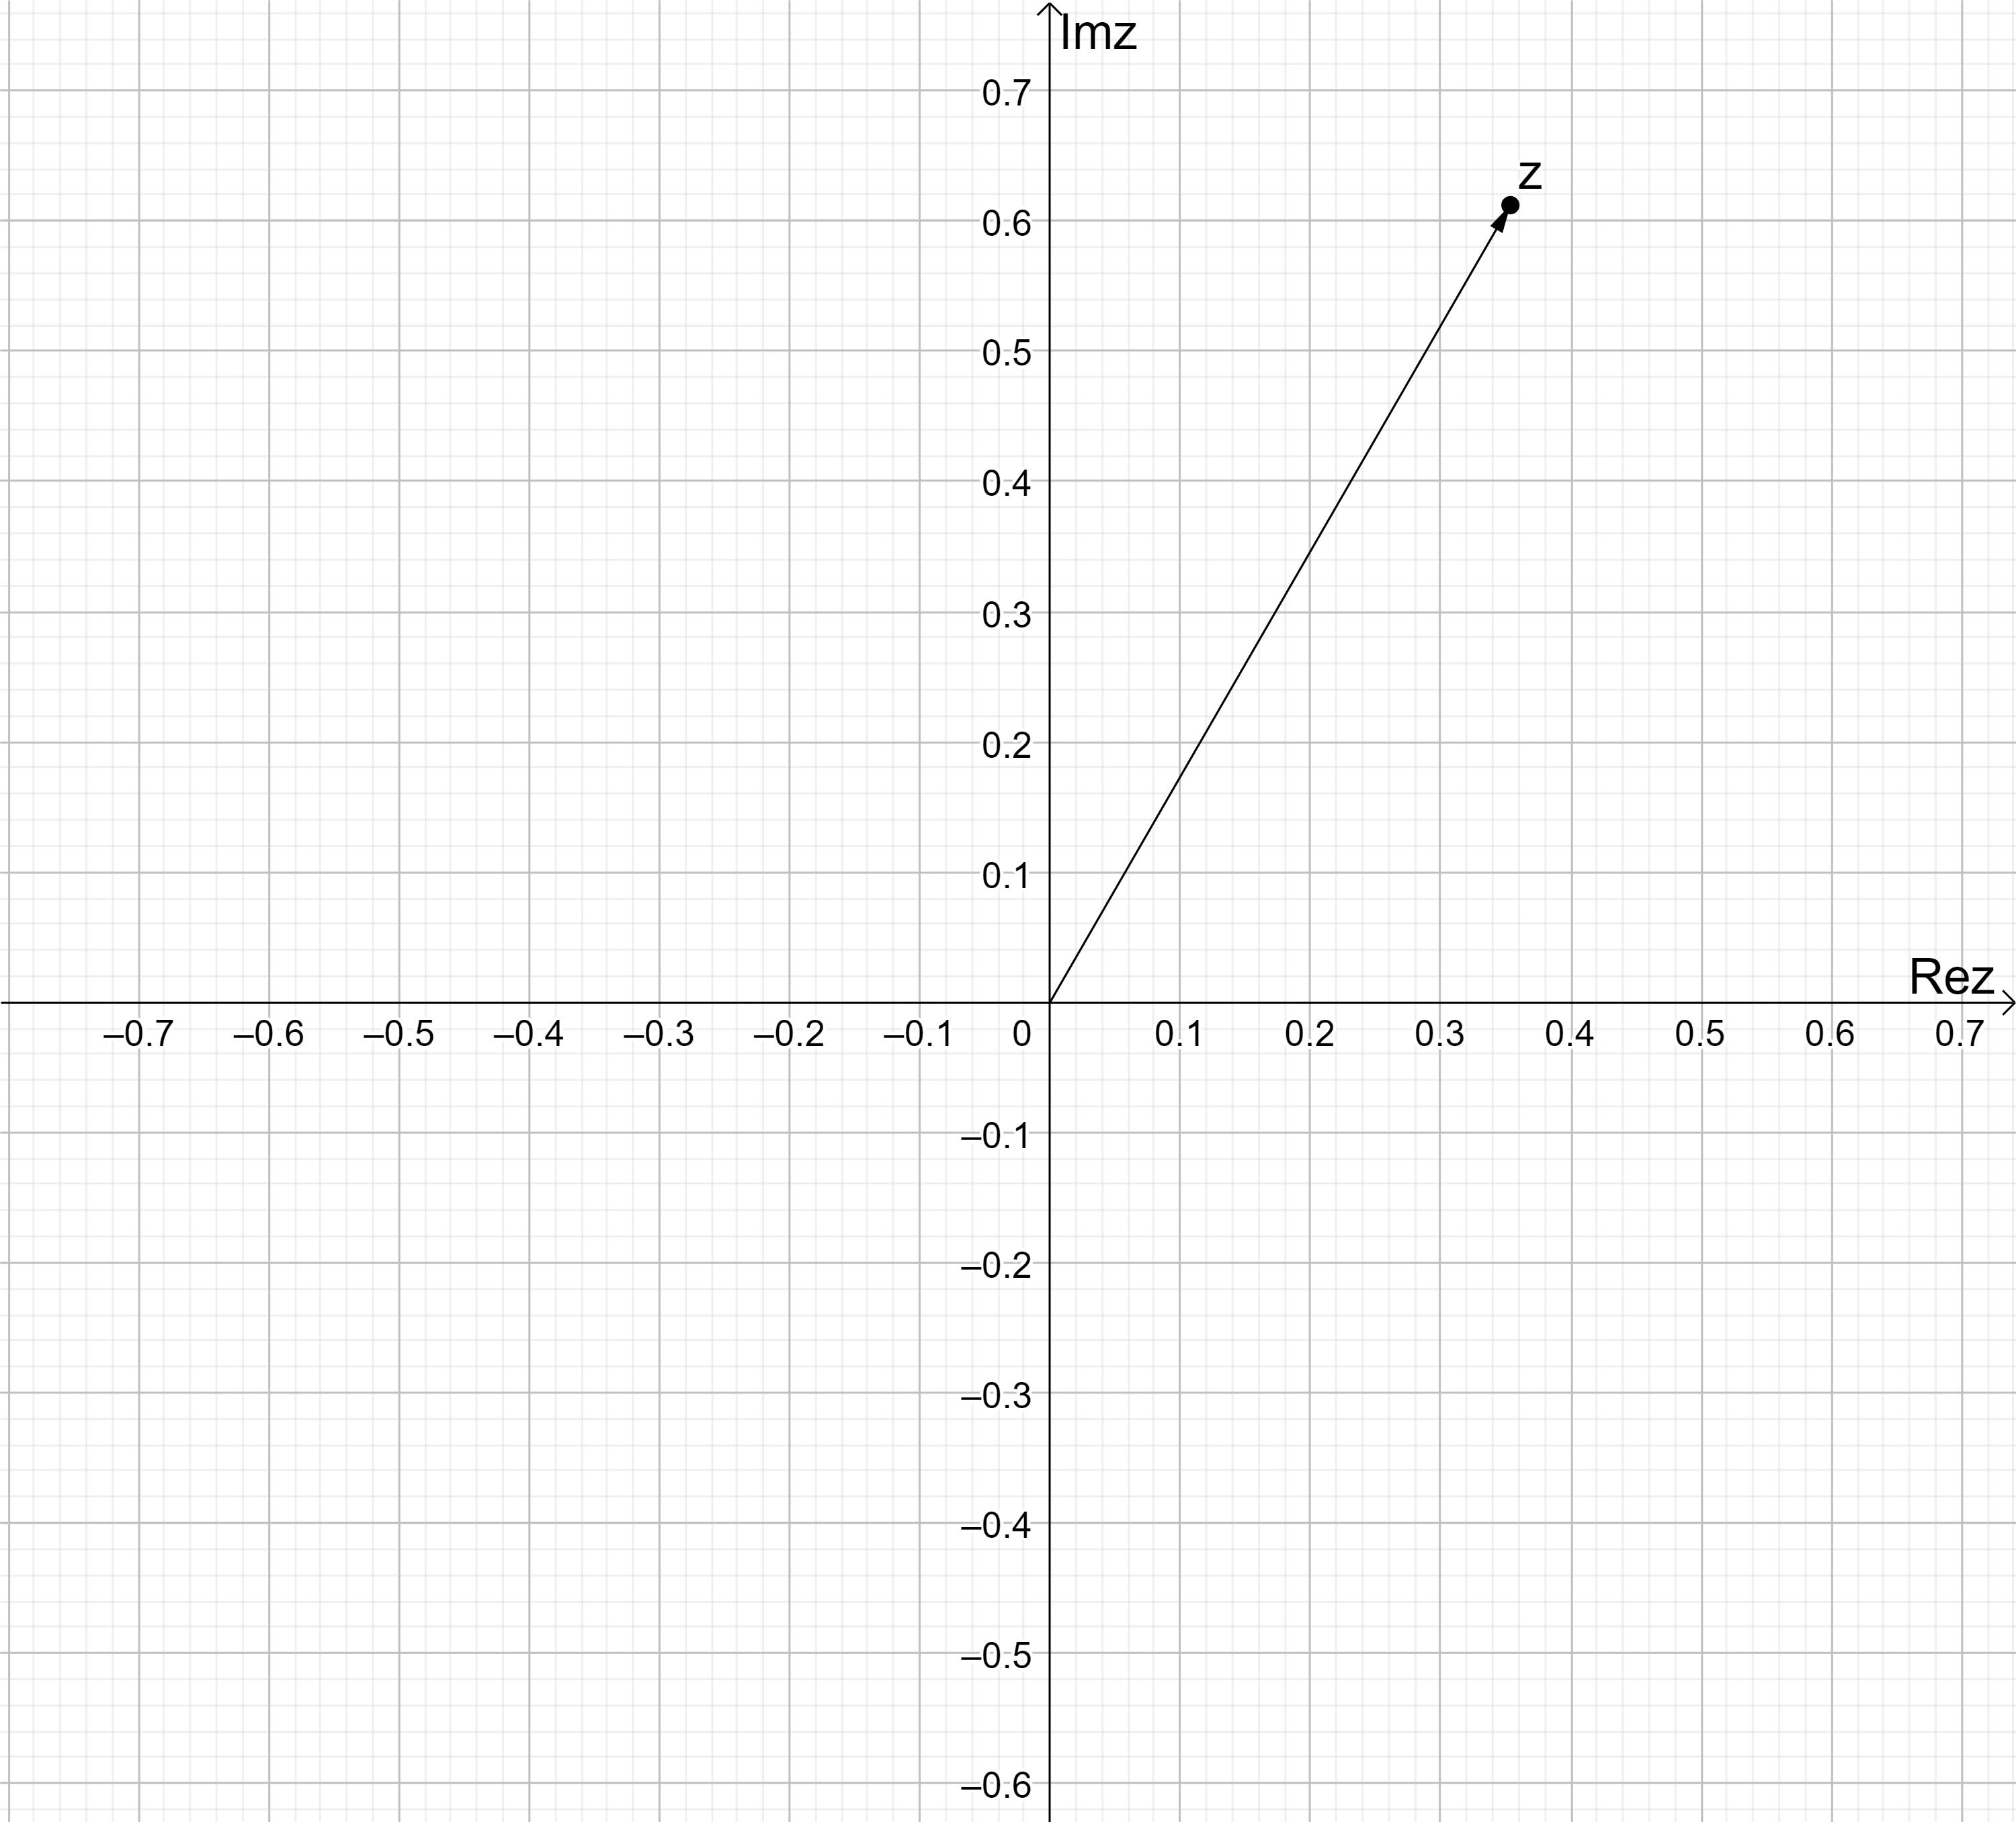
\includegraphics[width=0.6\textwidth]{task1-a.png}
            \caption{Изображение числа $z$ на комплексной плоскости}
        \end{figure}
        \item [б)]
        Для возведения числа $z$ в степень $n = 9$ воспользуемся 
        показательной формой записи.\\\\
        \begin{math}
            z^9 = (\frac{\sqrt{2}}{2}e^{i\frac{\pi}{3}})^9 = 
            \frac{\sqrt{2}}{2}e^{i9\frac{\pi}{3}} = 
            \frac{\sqrt{2}}{2}e^{i3\pi} =
            \frac{\sqrt{2}}{2}(\cos(3\pi) + i\sin(3\pi)) = 
            \frac{\sqrt{2}}{2}(-1 + 0) = -\frac{\sqrt{2}}{2}
        \end{math}\\   
        \item [в)]
        Для решения уравнения $w^3 = z$ извлечём из числа $z$ 
        комплексный корень:\\
        \begin{math}
            \newline      
            w^3 = z \\ w_k = (\sqrt[3]{z})_k ;  k = \overline{0,2}\\       
            w_k = \sqrt[3]{\frac{\sqrt{2}}{2}}e^{i\frac{1}{3}(\frac{\pi}{3} + 2\pi k)} ; k = \overline{0,2}\\
            w_k = \sqrt[3]{\frac{1}{\sqrt{2}}}e^{i(\frac{\pi}{3\cdot3} + \frac{2\pi k}{3})} ; k = \overline{0,2}\\ 
            w_k = \frac{1}{\sqrt[6]{2}}e^{i(\frac{\pi}{9} + \frac{2\pi k}{3})}.
        \end{math} \\\\
        Теперь вычислим корни для конкретных k:
        \begin{enumerate}
            \item [$k = 0:$] 
            \begin{math}
                w_0 = \frac{1}{\sqrt[6]{2}}{2}e^{i(\frac{\pi}{9} + \frac{2\pi \cdot0}{3})} = 
                \frac{1}{\sqrt[6]{2}}e^{i\frac{\pi}{9}}
            \end{math}
            \item [$k = 1:$]
            \begin{math}
                w_1 = \frac{1}{\sqrt[6]{2}}e^{i(\frac{\pi}{9} + \frac{2\pi \cdot1}{3})} = 
                \frac{1}{\sqrt[6]{2}}e^{i(\frac{\pi}{9} + \frac{6\pi}{9})} = 
                \frac{1}{\sqrt[6]{2}}e^{i\frac{7\pi}{9}}
            \end{math}
            \item [$k = 2:$]
            \begin{math}
                w_2 = \frac{1}{\sqrt[6]{2}}e^{i(\frac{\pi}{9} + \frac{2\pi \cdot2}{3})} =
                \frac{1}{\sqrt[6]{2}}e^{i(\frac{\pi}{9} + \frac{4\pi}{3})} = 
                \frac{1}{\sqrt[6]{2}}e^{i(\frac{\pi}{9} + \frac{12\pi}{9})} = 
                \frac{1}{\sqrt[6]{2}}e^{i\frac{13\pi}{9}}
            \end{math}\\\\
        \end{enumerate}
            \begin{figure}[h]
                \centering
                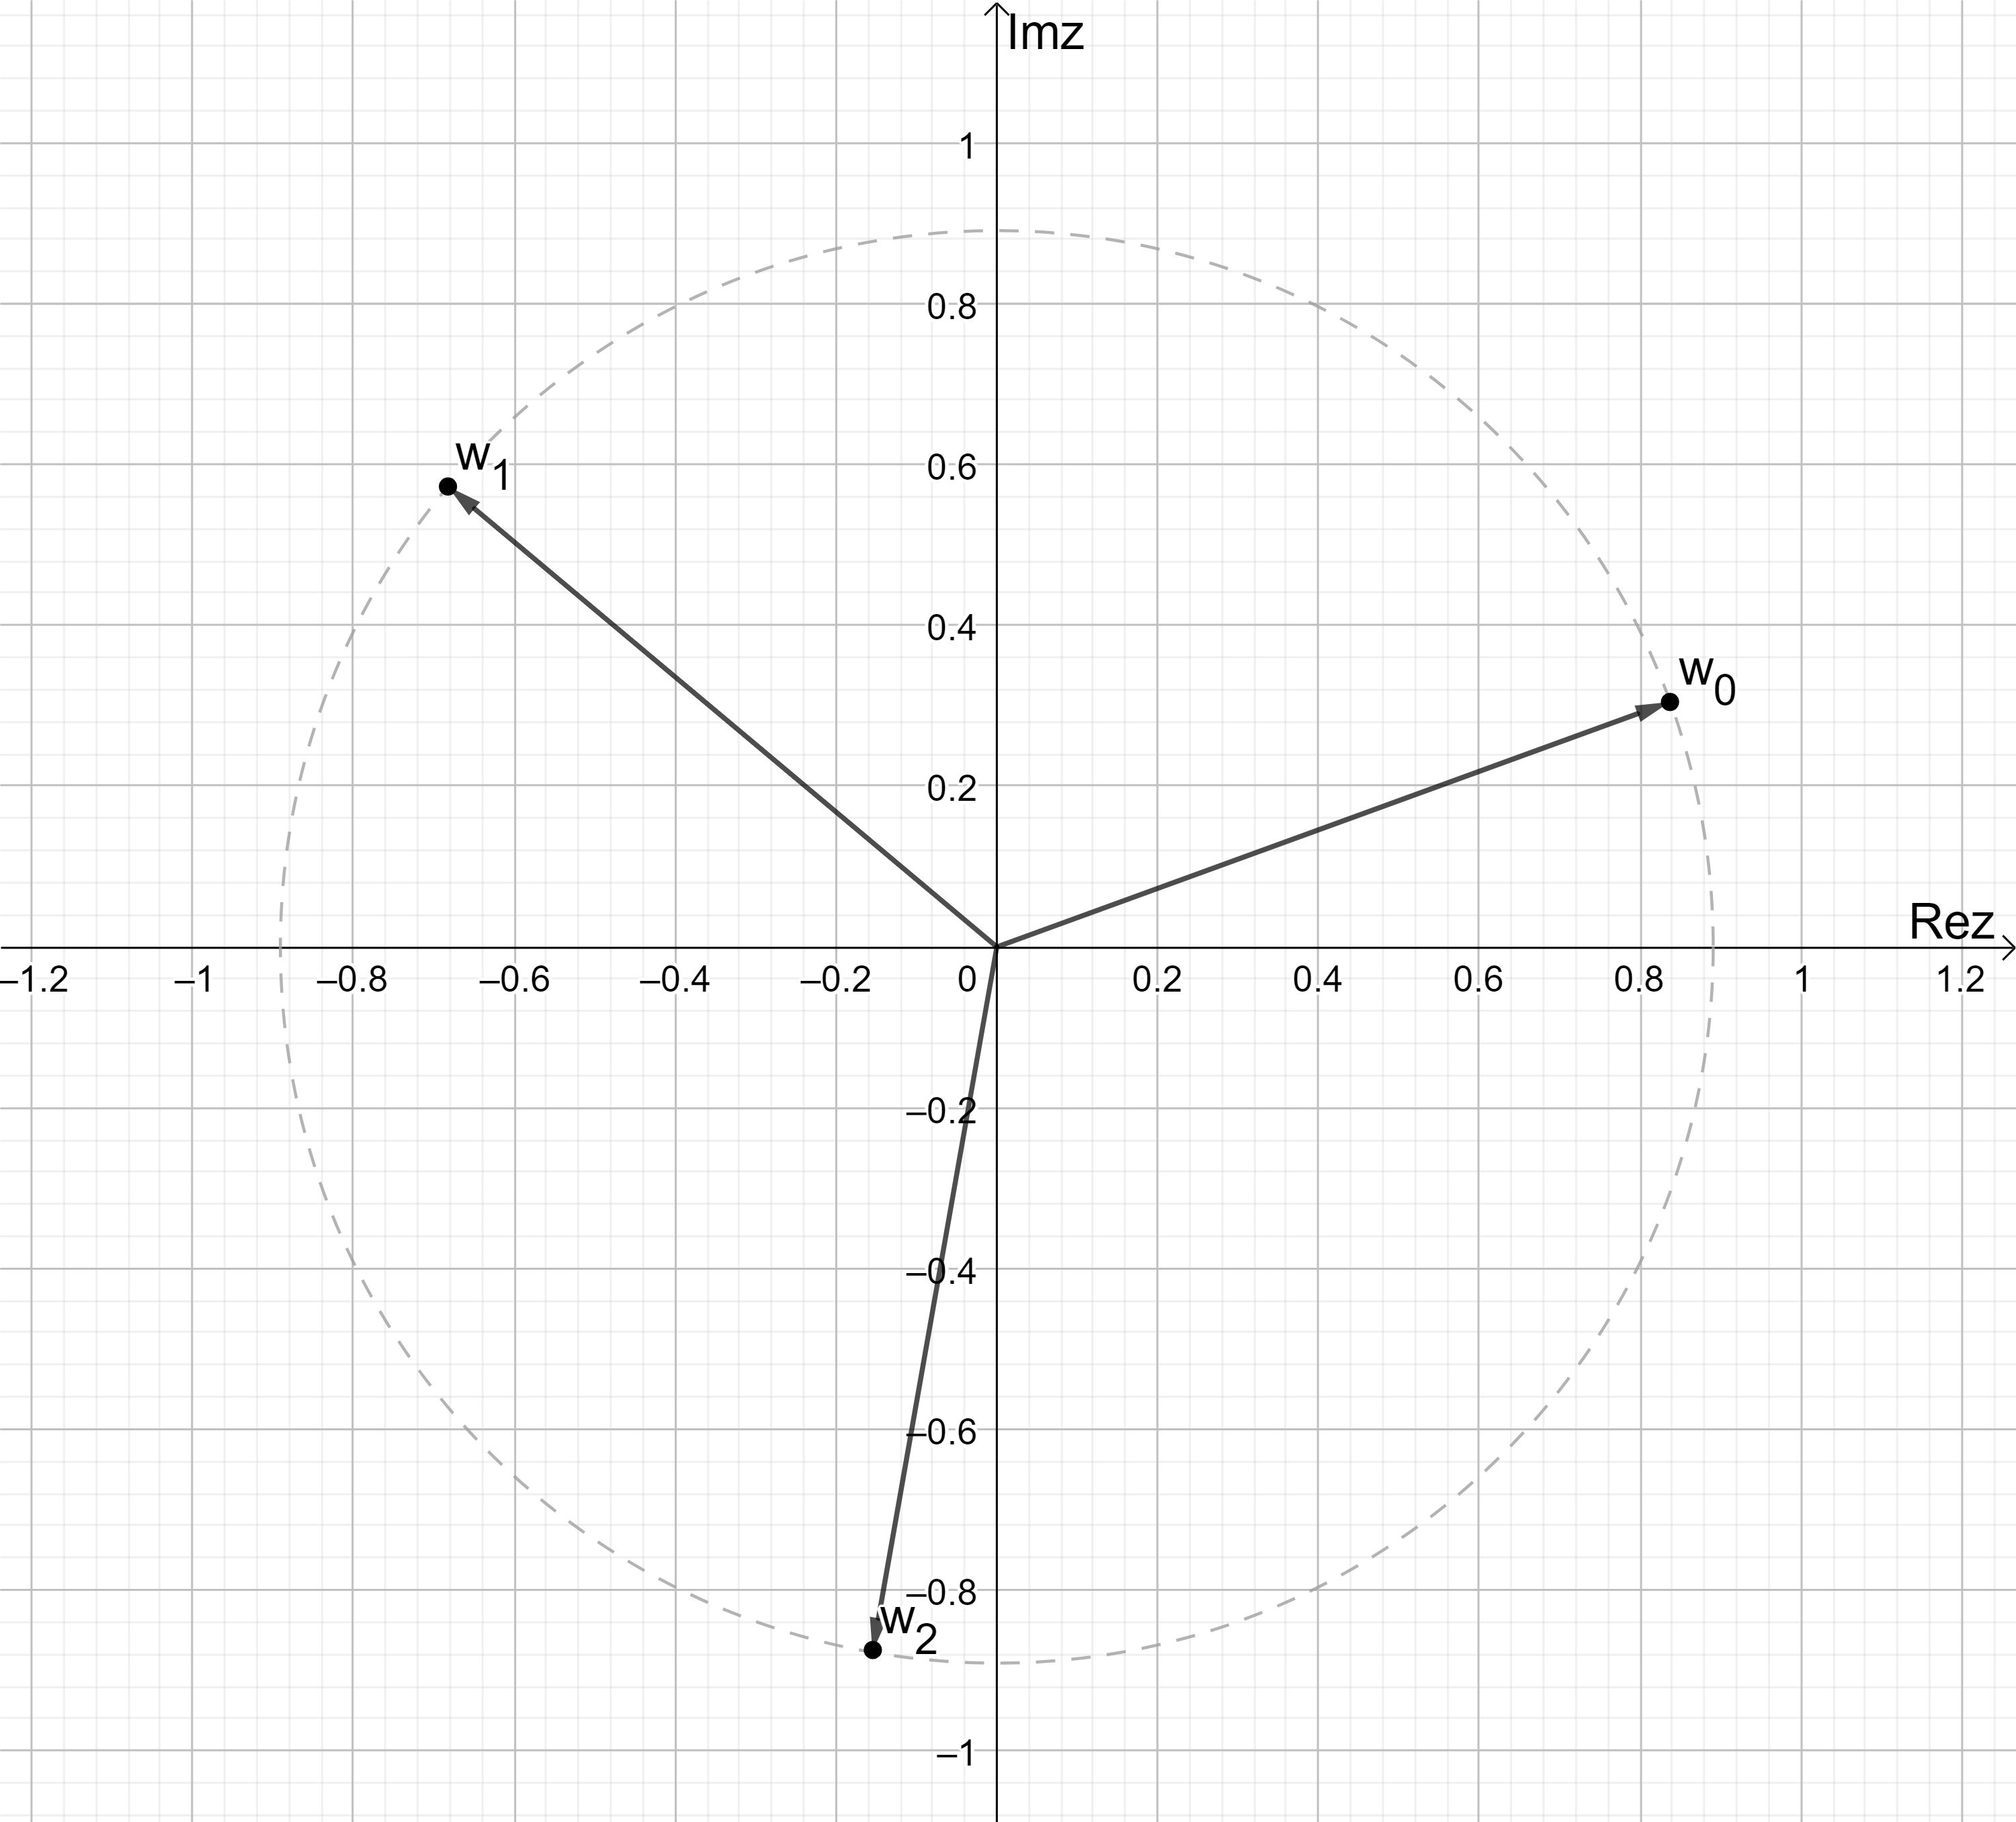
\includegraphics[width=0.65\textwidth]{task1-b.png}
                \caption{Изображение $\sqrt[3]{z}$ на комплексной плоскости}
            \end{figure}
            Убедимся в правильности найденных корней путём перемножения их
            друг на друга:\\
            \begin{math}
                w_0 \cdot w_1 \cdot w_2 = \frac{1}{\sqrt[6]{2}}e^{i\frac{\pi}{9}} \cdot
                \frac{1}{\sqrt[6]{2}}e^{i\frac{7\pi}{9}} \cdot
                \frac{1}{\sqrt[6]{2}}e^{i\frac{13\pi}{9}} = 
                \frac{1}{\sqrt[6]{2}\cdot\sqrt[6]{2}\cdot\sqrt[6]{2}}
                e^{(i\frac{\pi}{9} + i\frac{7\pi}{9} + i\frac{13\pi}{9})} = \\ =
                \frac{1}{(\sqrt[6]{2})^3}e^{i(\frac{\pi}{9} + \frac{7\pi}{9} + \frac{13\pi}{9})} = 
                \frac{1}{\sqrt{2}}e^{i\frac{\pi + 7\pi + 13\pi}{9}} = 
                \frac{1}{\sqrt{2}}e^{i\frac{21\pi}{9}} = 
                \frac{1}{\sqrt{2}}e^{i(2\pi + \frac{3\pi}{9})} = 
                \frac{1}{\sqrt{2}}e^{i\frac{\pi}{3}}
            \end{math}
            - результат совпал с числом $z$, значит корни уравнения найдены верно.      
    \end{enumerate}
    \subsection*{Ответ:}
    \begin{enumerate}
        \item [а)] 
        Алгебраическая форма записи: 
        $z = \frac{\sqrt{2}}{4}(1 + i\sqrt{3})$.\\
        Тригонометрическая форма записи: 
        $z = \frac{\sqrt{2}}{2}(\cos(\frac{\pi}{3}) + i\sin(\frac{\pi}{3}))$.\newline
        Показательная форма записи:
        $z = \frac{\sqrt{2}}{2}e^{i\frac{\pi}{3}}$.\\
        \item [б)] $z^9 = -\frac{\sqrt{2}}{2}$
        \item [в)] $w_0 = \frac{1}{\sqrt[6]{2}}e^{i\frac{\pi}{9}}$\newline
        $w_1 = \frac{1}{\sqrt[6]{2}}e^{i\frac{7\pi}{9}}$\\
        $w_2 = \frac{1}{\sqrt[6]{2}}e^{i\frac{13\pi}{9}}$\\
    \end{enumerate}
%--------------------------------------
%
% 2 задание
%
%--------------------------------------
\section{Задание.}
    Изобразить на плоскости:\\\\
    $\Re e(\frac{i}{z}) - \frac{\Im m(iz)}{z\overline{z}} = 0$
    \subsection*{Решение:}
    Поскольку $z$ и $\overline{z}$ в знаменателе, они не должны быть равны 0,
    то есть $\Re ez \neq 0$ и $\Im mz \neq 0$, или $|z| \neq 0$.\newline
    Так же вспомним, что по свойствам комплесных чисел $z\overline{z} = |z|^2$\newline
    \begin{math} 
        \Re e(\frac{i}{z}) - \frac{\Im m(iz)}{z\overline{z}} = 0 \Leftrightarrow
        \Re e(\frac{i\overline{z}}{z\overline{z}}) - \frac{\Im m(iz)}{z\overline{z}} = 0 \Leftrightarrow
        \Re e(\frac{i\overline{z}}{|z|^2}) - \frac{\Im m(iz)}{|z|^2} = 0 \Leftrightarrow
        \frac{\Re e(i\overline{z})}{|z|^2} - \frac{\Im m(iz)}{|z|^2} = 0 \Leftrightarrow
        \Re e(i\overline{z}) - \Im m(iz) = 0.
    \end{math} \\\\
    Пусть $z = x + iy$. Тогда:\\
    \begin{math}
        \begin{cases}
            x \neq 0\\
            y \neq 0
        \end{cases}\\
        \Re e(i\overline{(x + iy)}) - \Im m(i(x + iy)) = 0 \Leftrightarrow
        \Re e(i(x - iy)) - \Im m(ix - y) = 0 \Leftrightarrow
        \Re e(ix + y) - \Im m(ix - y) = 0 \Leftrightarrow
        y - x = 0 \Leftrightarrow
        y = x.
    \end{math}\\
    Графиком этой функции будет прямая с выколотой точкой $(0;0)$
    \begin{figure}[h]
        \centering
        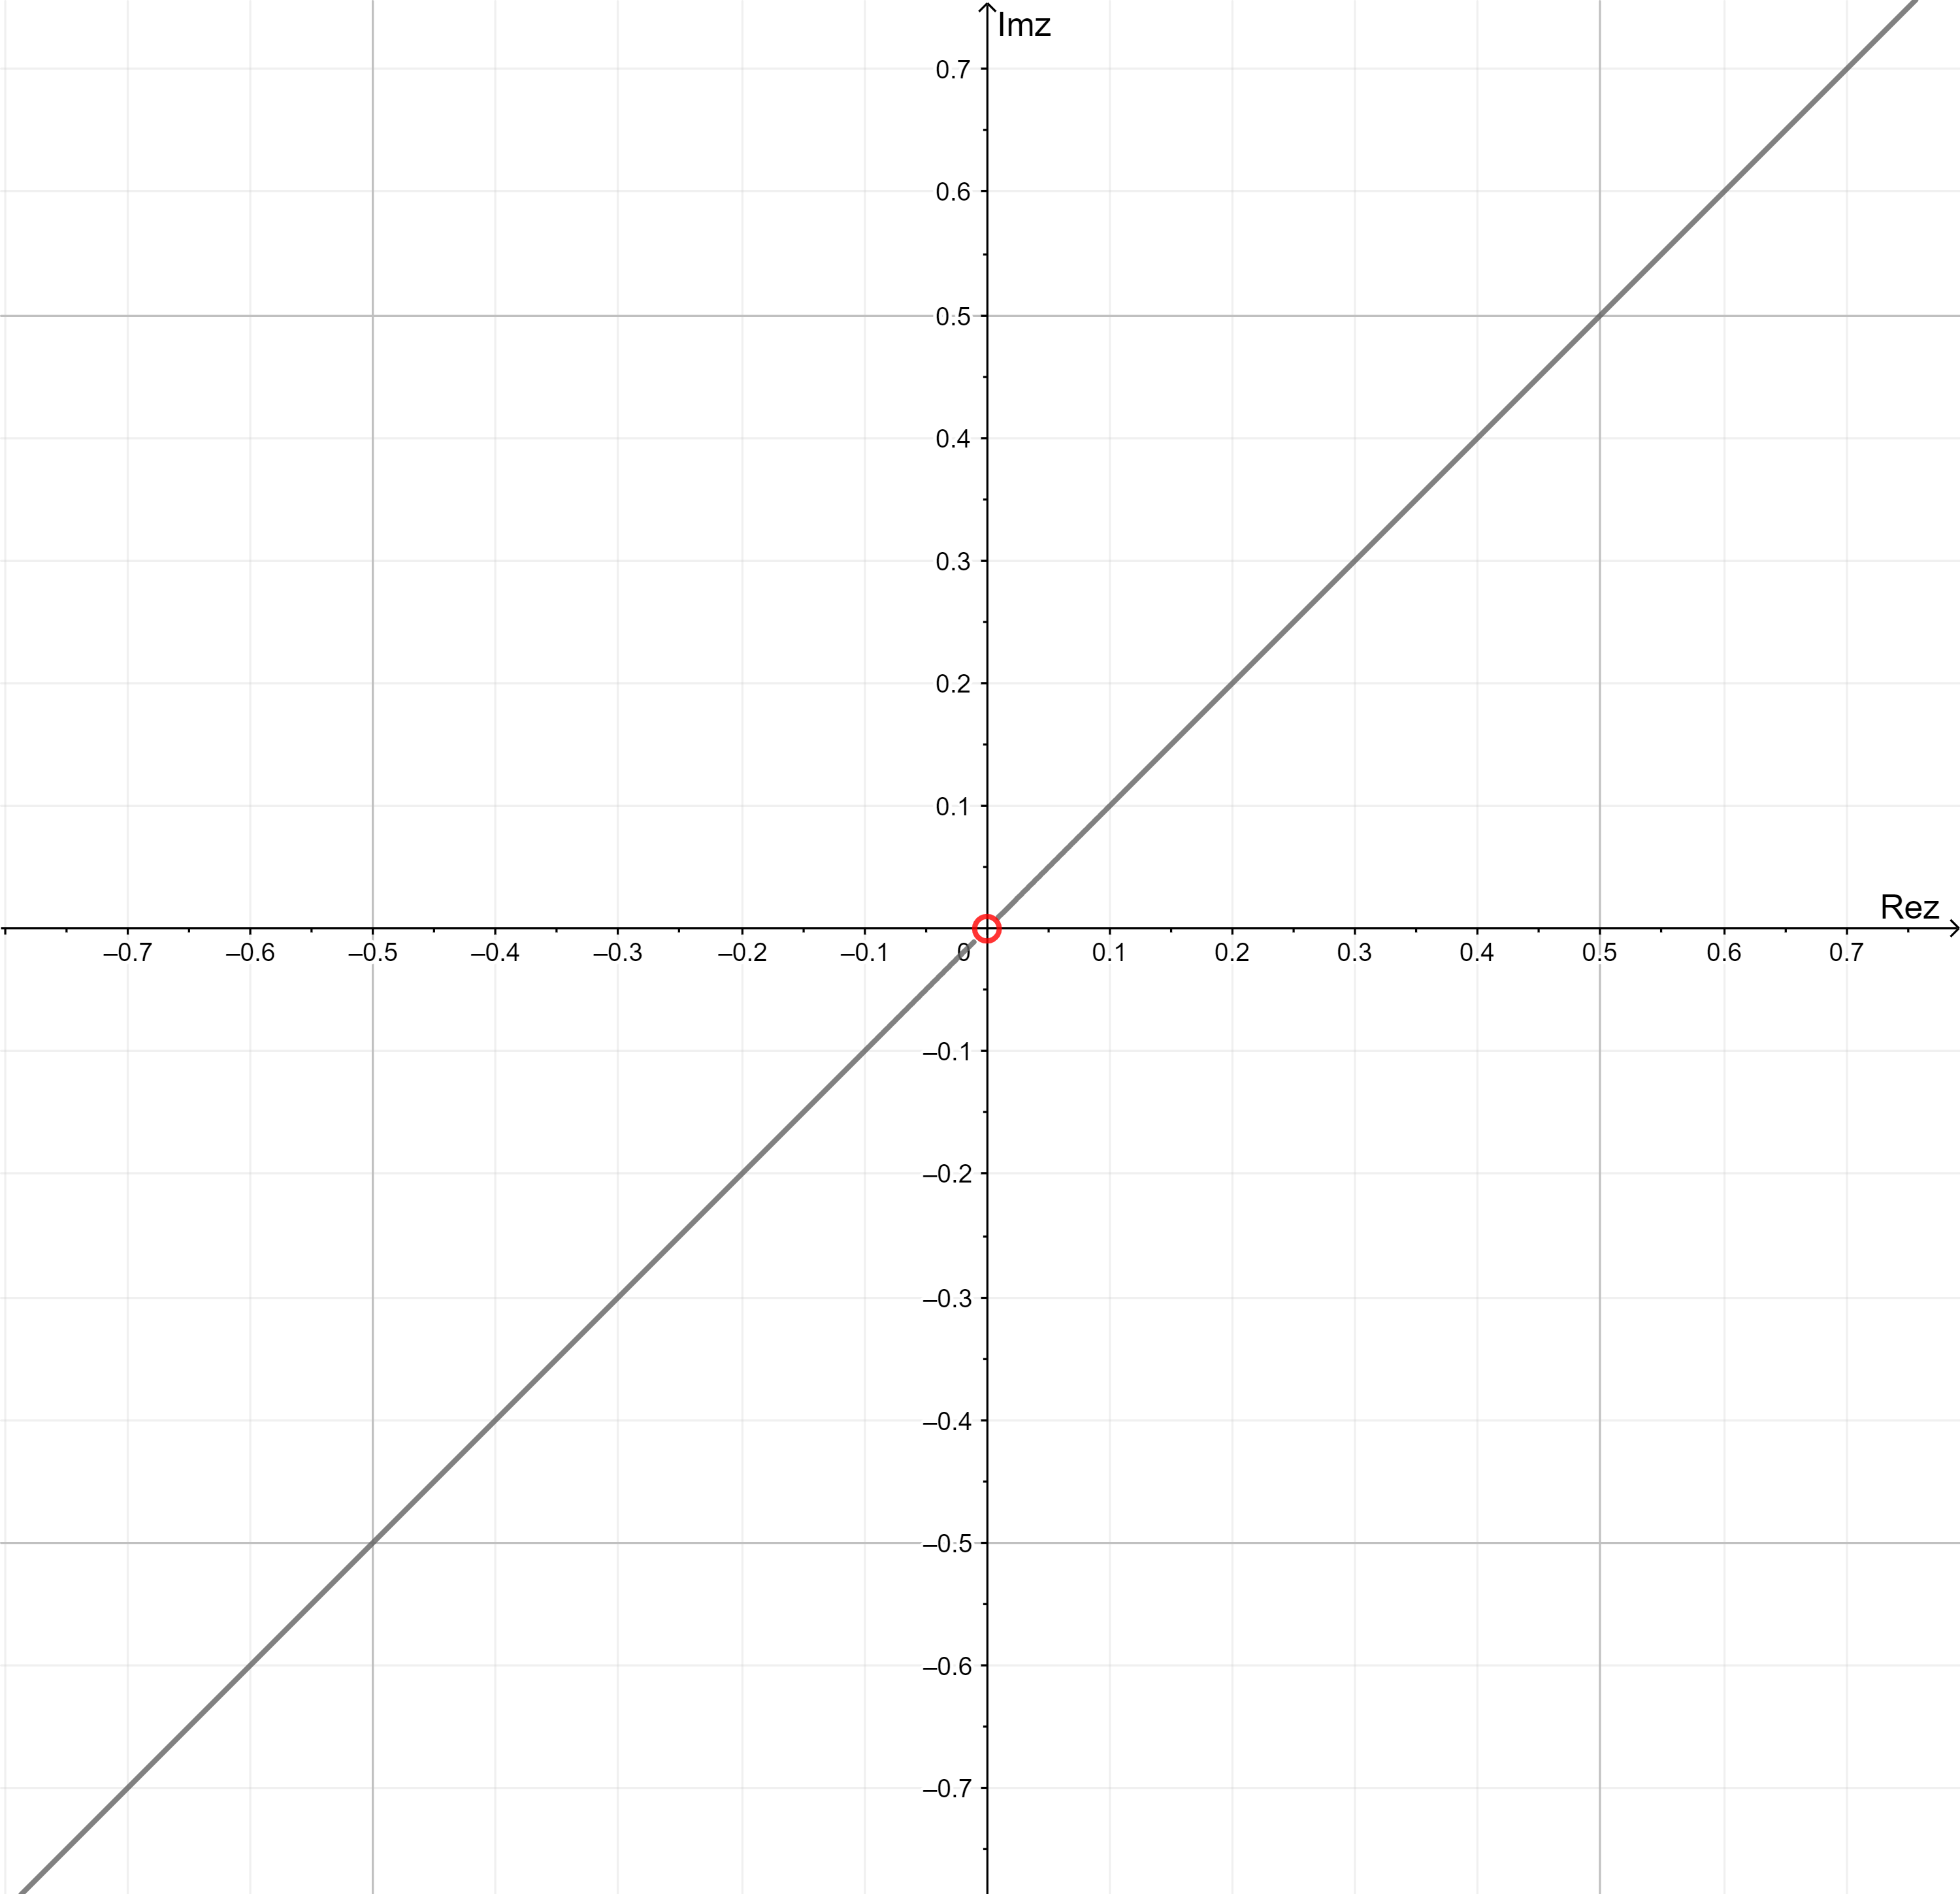
\includegraphics[width=0.63\textwidth]{task2-a.png}
        \caption{Изображение $\Re e(\frac{i}{z}) - \frac{\Im m(iz)}{z\overline{z}} = 0$ на плоскости}
    \end{figure}
%--------------------------------------
%
% 3 задание
%
%--------------------------------------
\newpage
\newpage
\section{Задание.} 
    Найти $x$ и $y$, считая их вещественными:\\\\
    $(-6 + i)x + (11 - 2i)y = 3 - 4i$\\
    \subsection*{Решение:}
    \begin{math}
        (-6 + i)x + (11 - 2i)y = 3 - 4i \Leftrightarrow\\
        \Leftrightarrow-6x + ix + 11y - 2iy = 3 - 4i \Leftrightarrow\\
        \Leftrightarrow-6x + 11y +i(x - 2y) = 3 - 4i \Leftrightarrow\\
        \Leftrightarrow
        \begin{cases}
            -6x + 11y = 3\\
            x - 2y = -4
        \end{cases}\Leftrightarrow
        \begin{cases}
            -6(2y - 4) + 11y = 3\\
            x = 2y - 4
        \end{cases}\Leftrightarrow
        \begin{cases}
            -12y + 24 + 11y = 3\\
            x = 2y - 4
        \end{cases}\Leftrightarrow\\\Leftrightarrow   
        \begin{cases}
           -y = -21\\
           x = 2y - 4 
        \end{cases}\Leftrightarrow
        \begin{cases}
            y = 21\\
            x = 2\cdot21 - 4
        \end{cases}\Leftrightarrow
        \begin{cases}
            y = 21\\
            x = 38
        \end{cases}
    \end{math}
    \subsection*{Ответ:} $x = 38;\\ y = 21$  
%--------------------------------------
%
% 4 задание
%
%--------------------------------------
\newpage
\newpage
\section{Задание.}
    Графически изобразить множества точек, удовлетворяющих следующим неравенствам:
    \begin{enumerate}
        \item [a)] $-4 \leq \Re ez \leq 2$
        \item [b)] $1 \leq \Im mz \leq 4$
        \item [c)] $2 < |z| \leq 5$
        \item [d)] $|z| < 3$
        \item [e)] $2 < |z + 3 - i| < 3$
        \item [f)] $\frac{5\pi}{4} < \phi < \frac{3\pi}{2}$
    \end{enumerate}\newpage
    \subsection*{Решение:}
    \begin{enumerate}
        \item [a)] $-4 \leq \Re ez \leq 2$\\
        Пусть $z = x + iy$. Тогда:\\
        $-4 \leq \Re e(x + iy) \leq 2 \Leftrightarrow$
        $-4 \leq x \leq 2$\\
        Графическим изображением данного неравенства будет вертикальная полоса.
        \begin{figure}[h]
            \centering
            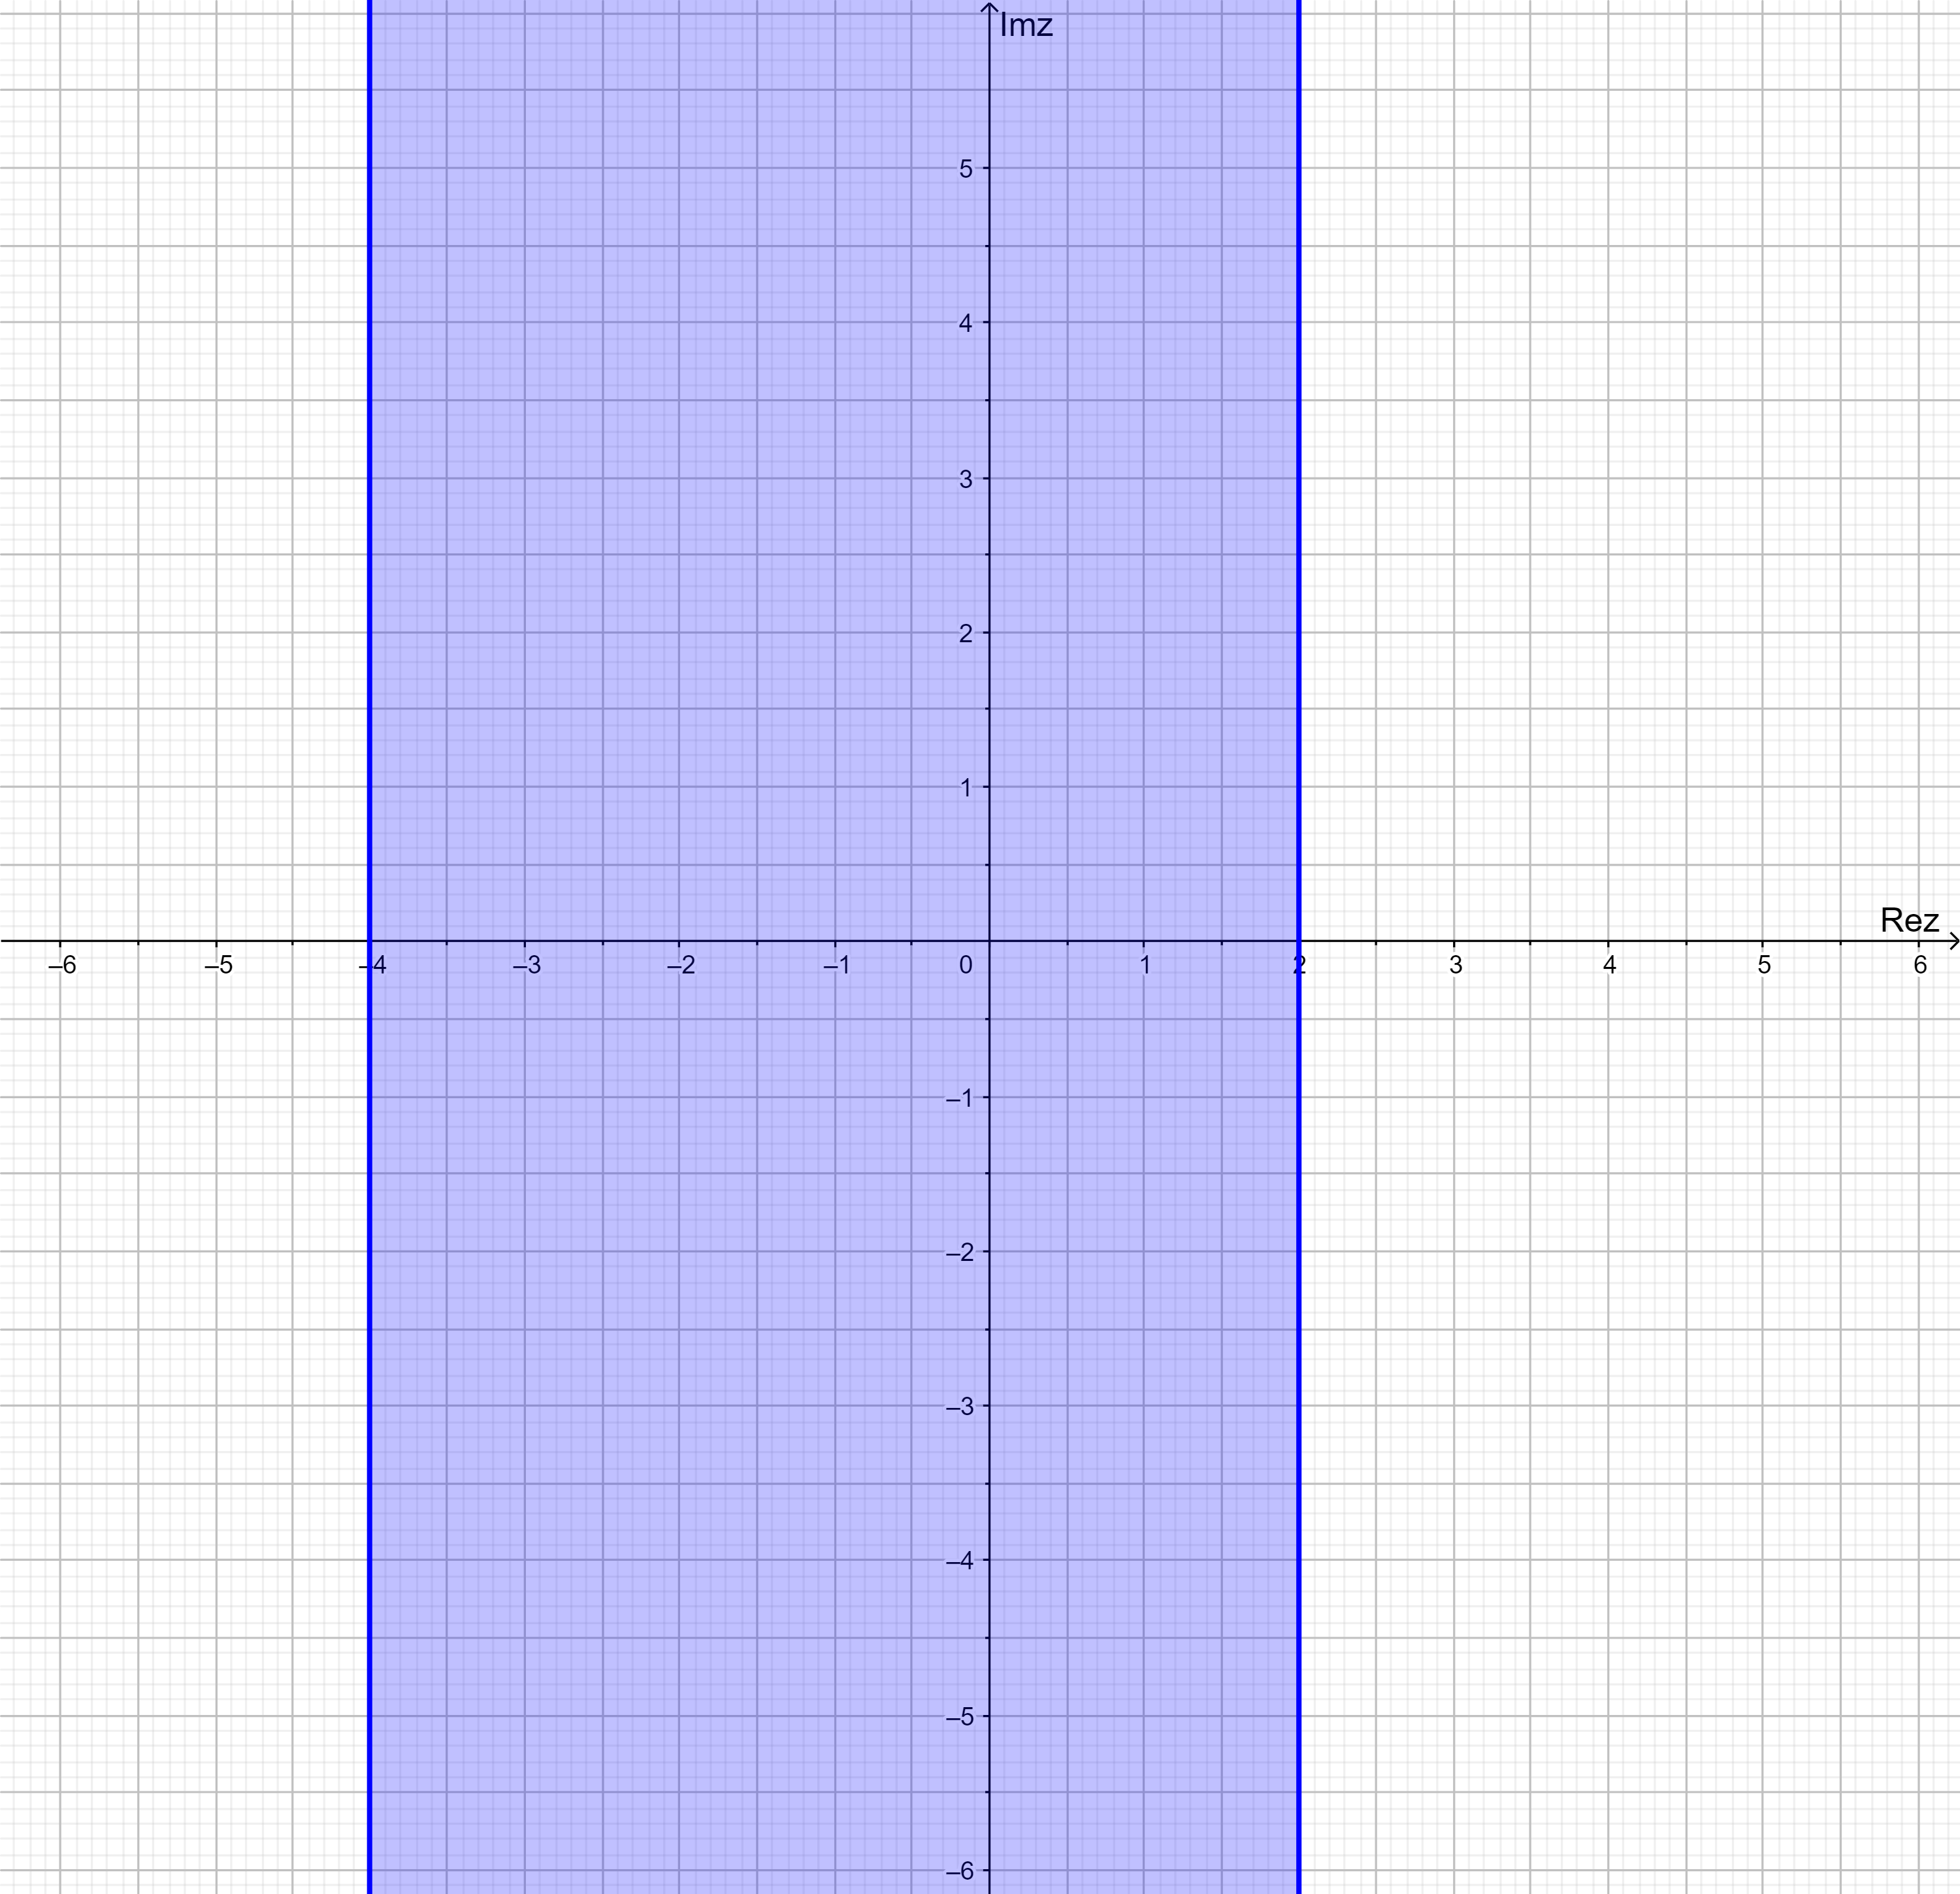
\includegraphics[width=0.75\textwidth]{task4-a.png}
            \caption{Графическое изображение $-4 \leq \Re ez \leq 2$}
        \end{figure}\newpage
        \item [b)] $1 \leq \Im mz \leq 4$\\
        Пусть $z = x + iy$. Тогда:\\
        $1 \leq \Im m(x + iy) \leq 4 \Leftrightarrow$
        $1 \leq y \leq 4$\\
        Графическим изображением данного неравенства будет горизонтальная полоса.\\
        \begin{figure}[h]
            \centering
            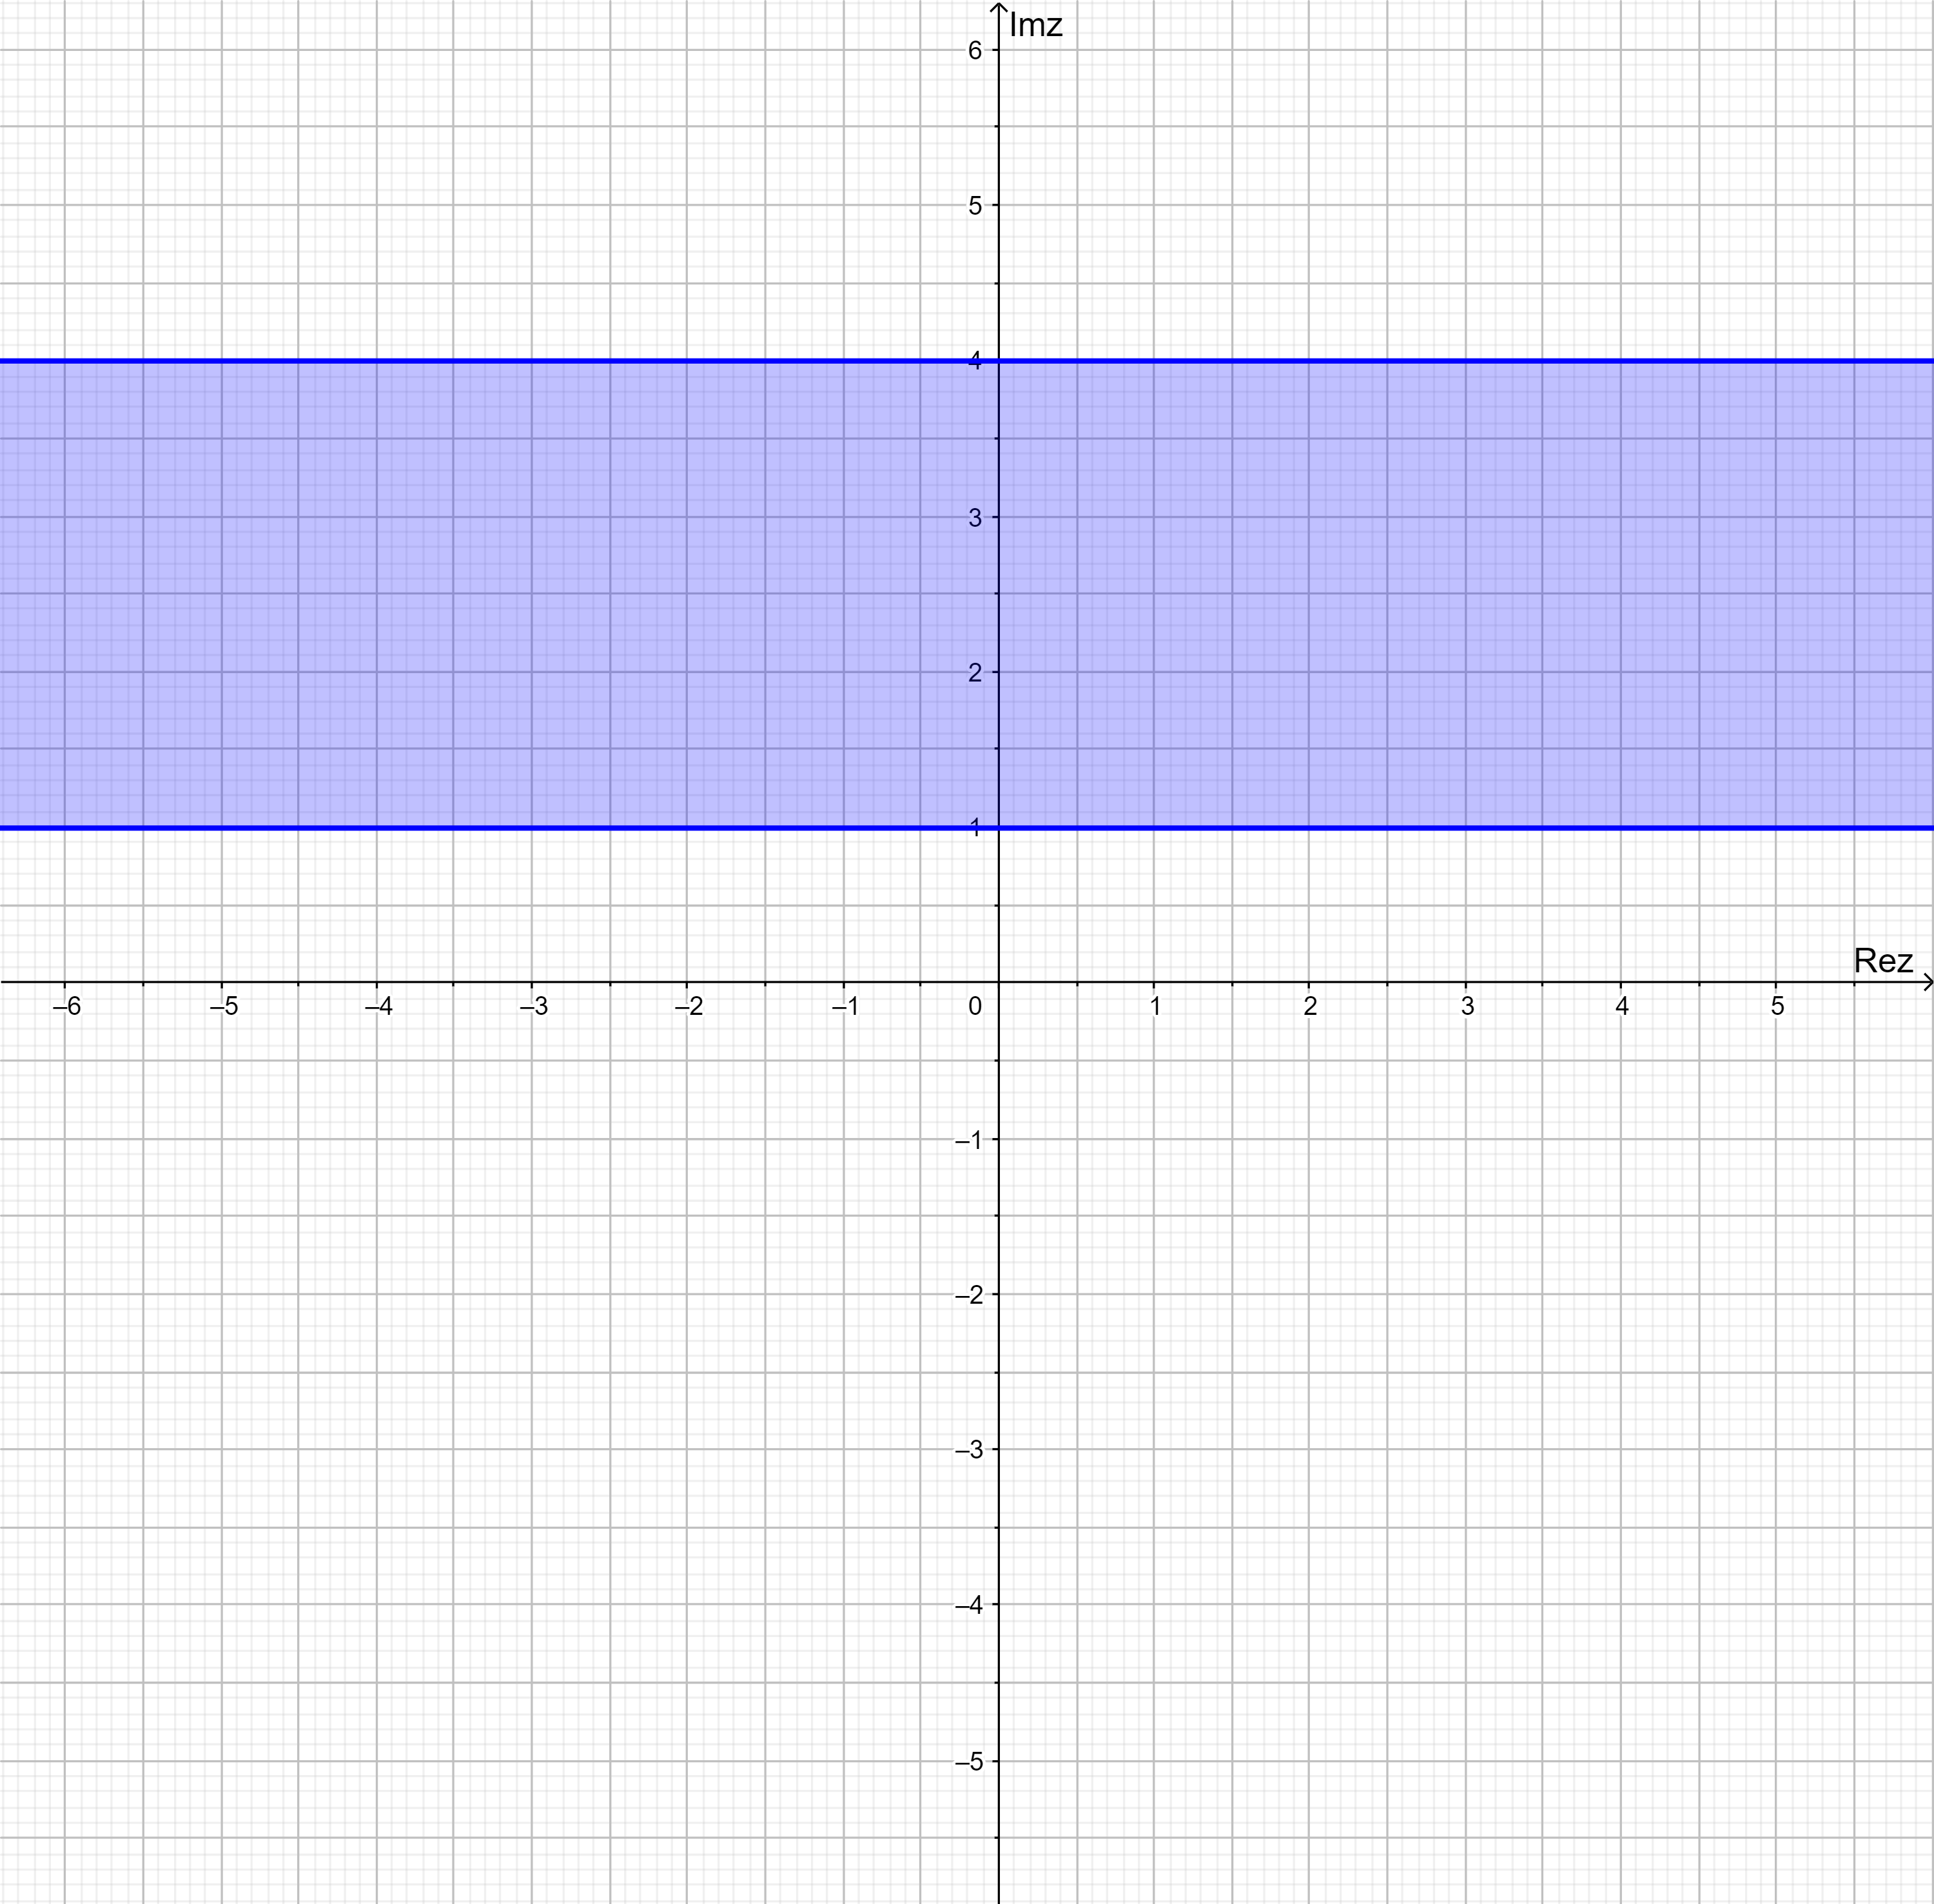
\includegraphics[width=0.75\textwidth]{task4-b.png}
            \caption{Графическое изображение $1 \leq \Im mz \leq 4$}
        \end{figure}\newpage
        \item [c)] $2 < |z| \leq 5$\\
        Пусть $z = x + iy$. Тогда:\\
        \begin{math}
            2 < |z| \leq 5 \Leftrightarrow
            2 < \sqrt{x^2 + y^2} \leq 5\Leftrightarrow
            2^2 < x^2 + y^2 \leq 5^2 \Leftrightarrow\\\Leftrightarrow
            4 < x^2 + y^2 \leq 25.
        \end{math}\\
        Графическим изображением данного неравенства будет кольцо,
        у которого малый радиус равен 2, а больший радиус равен 5.\\
        \begin{figure}[h]
            \centering
            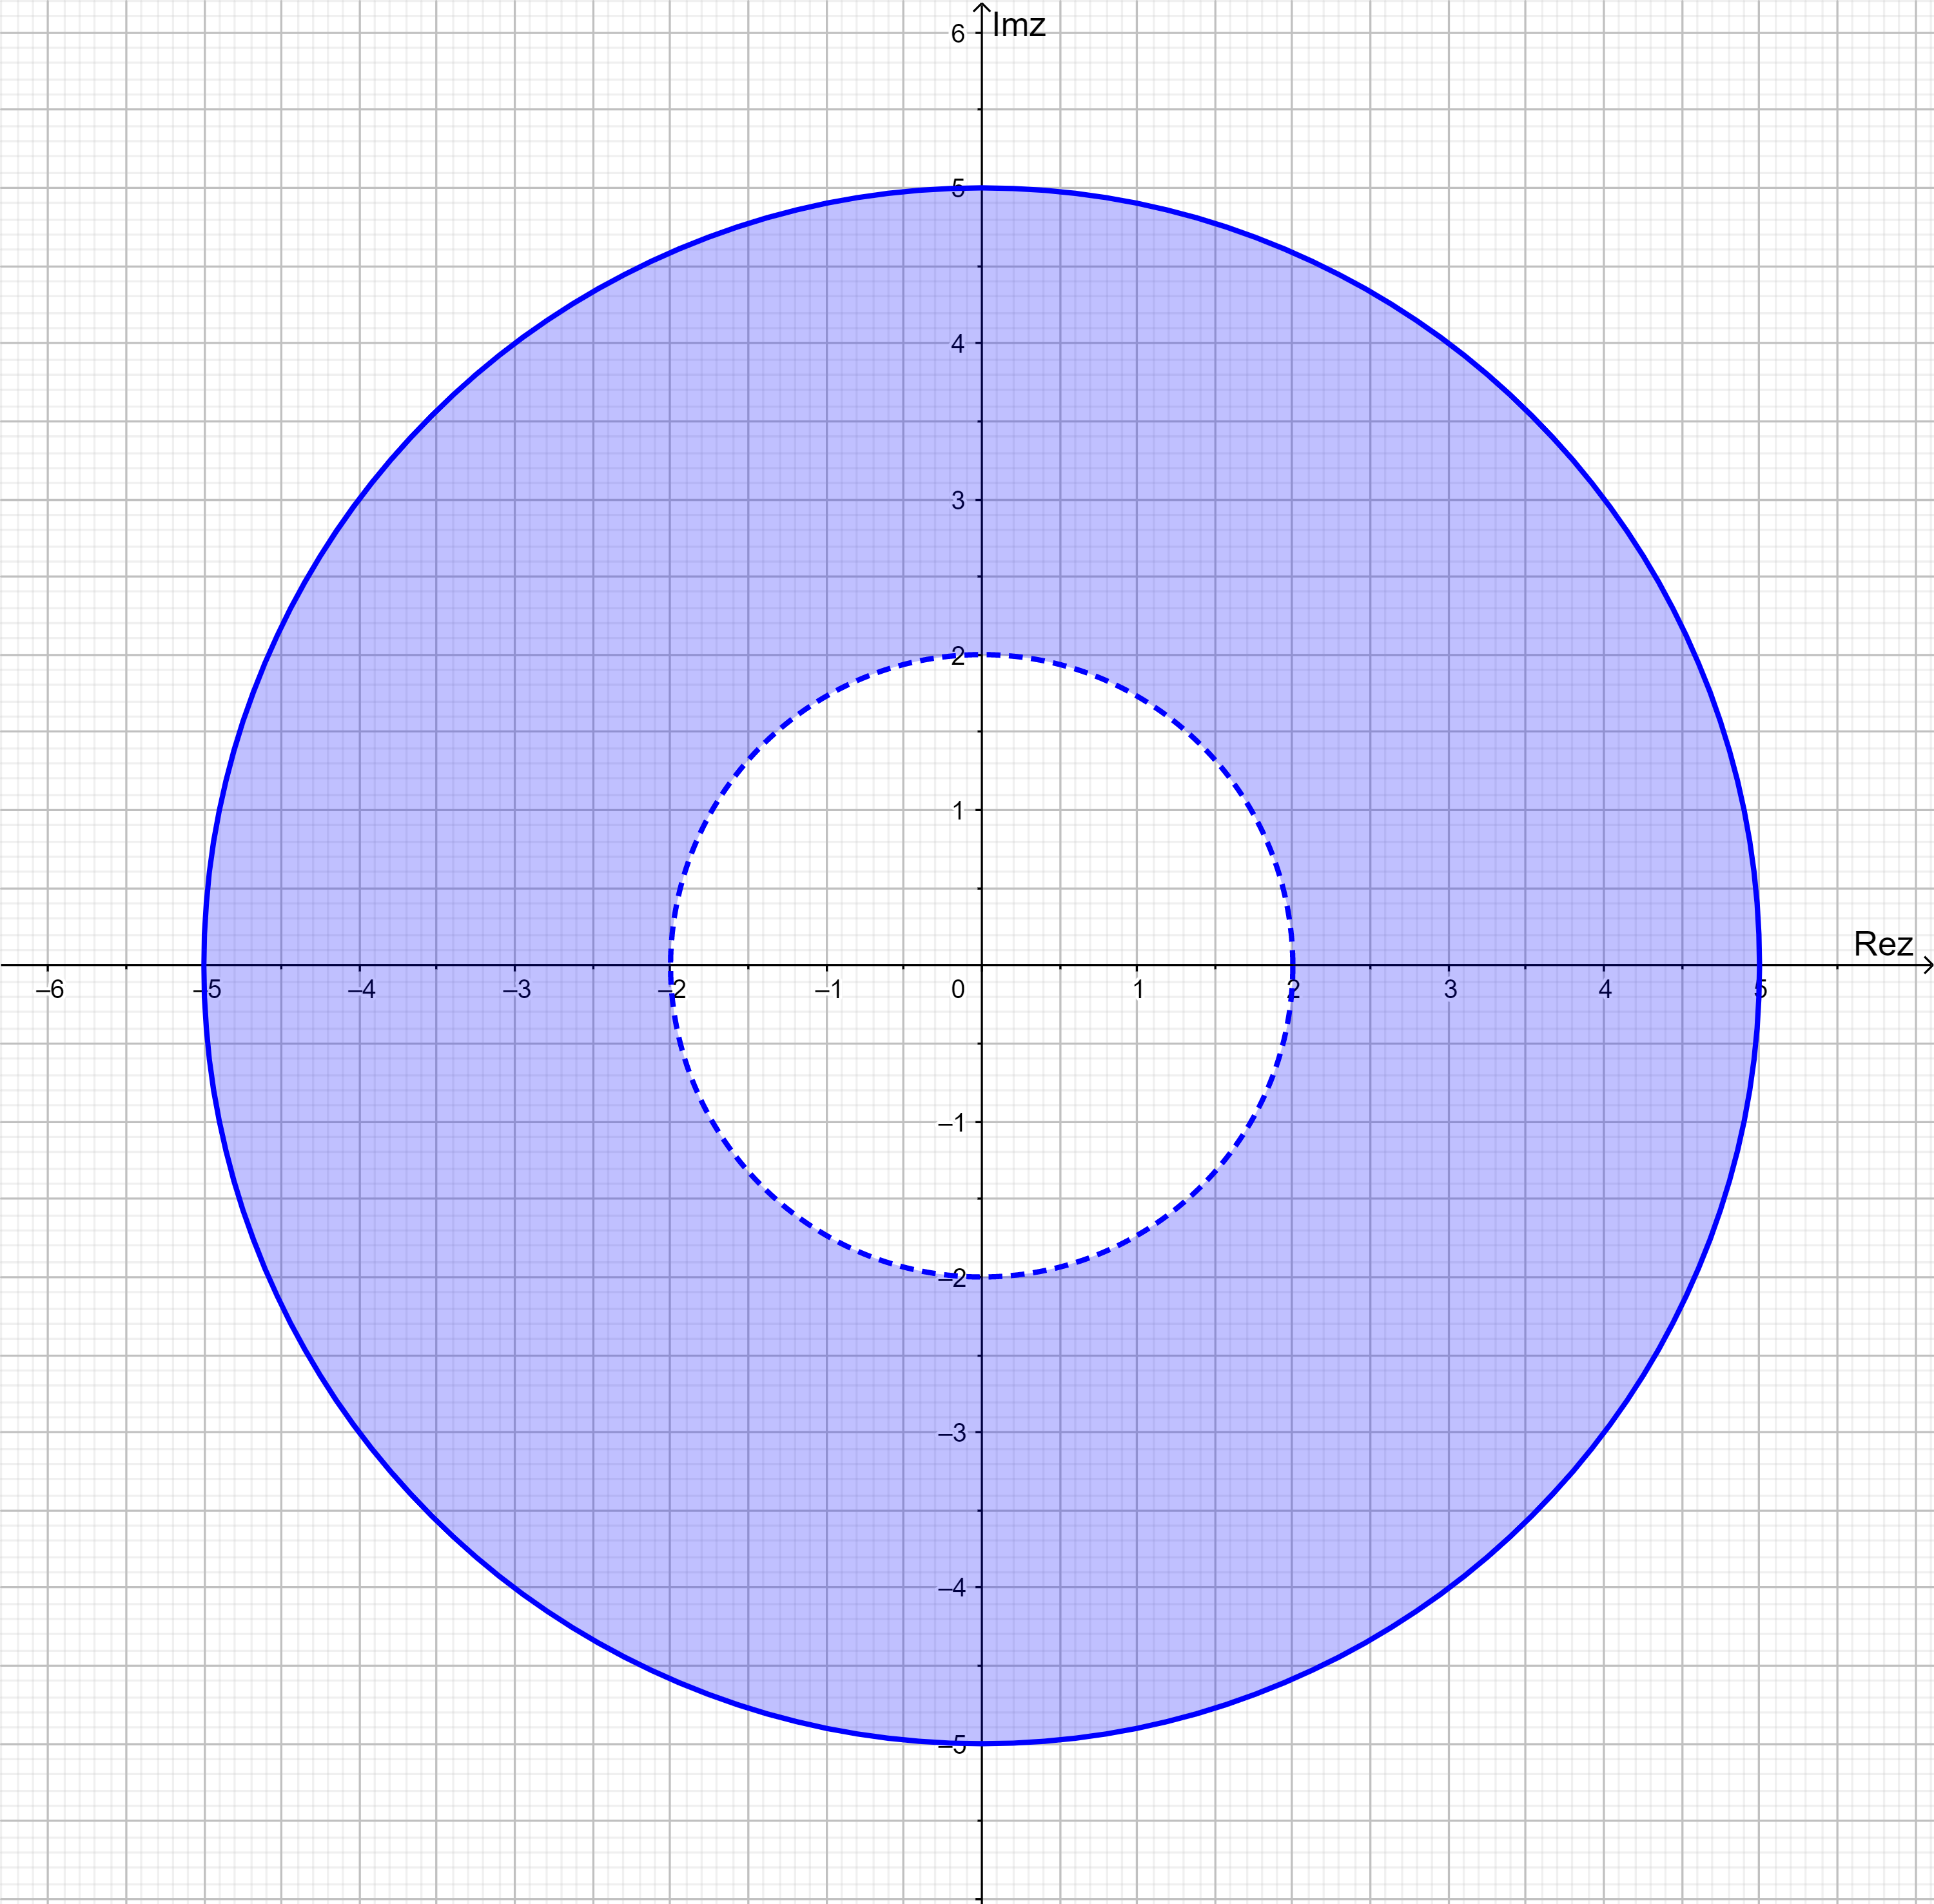
\includegraphics[width=0.75\textwidth]{task4-c.png}
            \caption{Графическое изображение $2 < |z| \leq 5$}
        \end{figure}\newpage
        \item [d)] $|z| < 3$\\
        Пусть $z = x + iy$. Тогда:\\
        \begin{math}
            |z| < 3 \Leftrightarrow
            \sqrt{x^2 + y^2} < 3 \Leftrightarrow
            x^2 + y^2 < 3^2 \Leftrightarrow\\\Leftrightarrow
            x^2 + y^2 < 9.
        \end{math}\\
        Графическим изображением данного неравенства будет
        круг с радиусом 3.\\
        \begin{figure}[h]
            \centering
            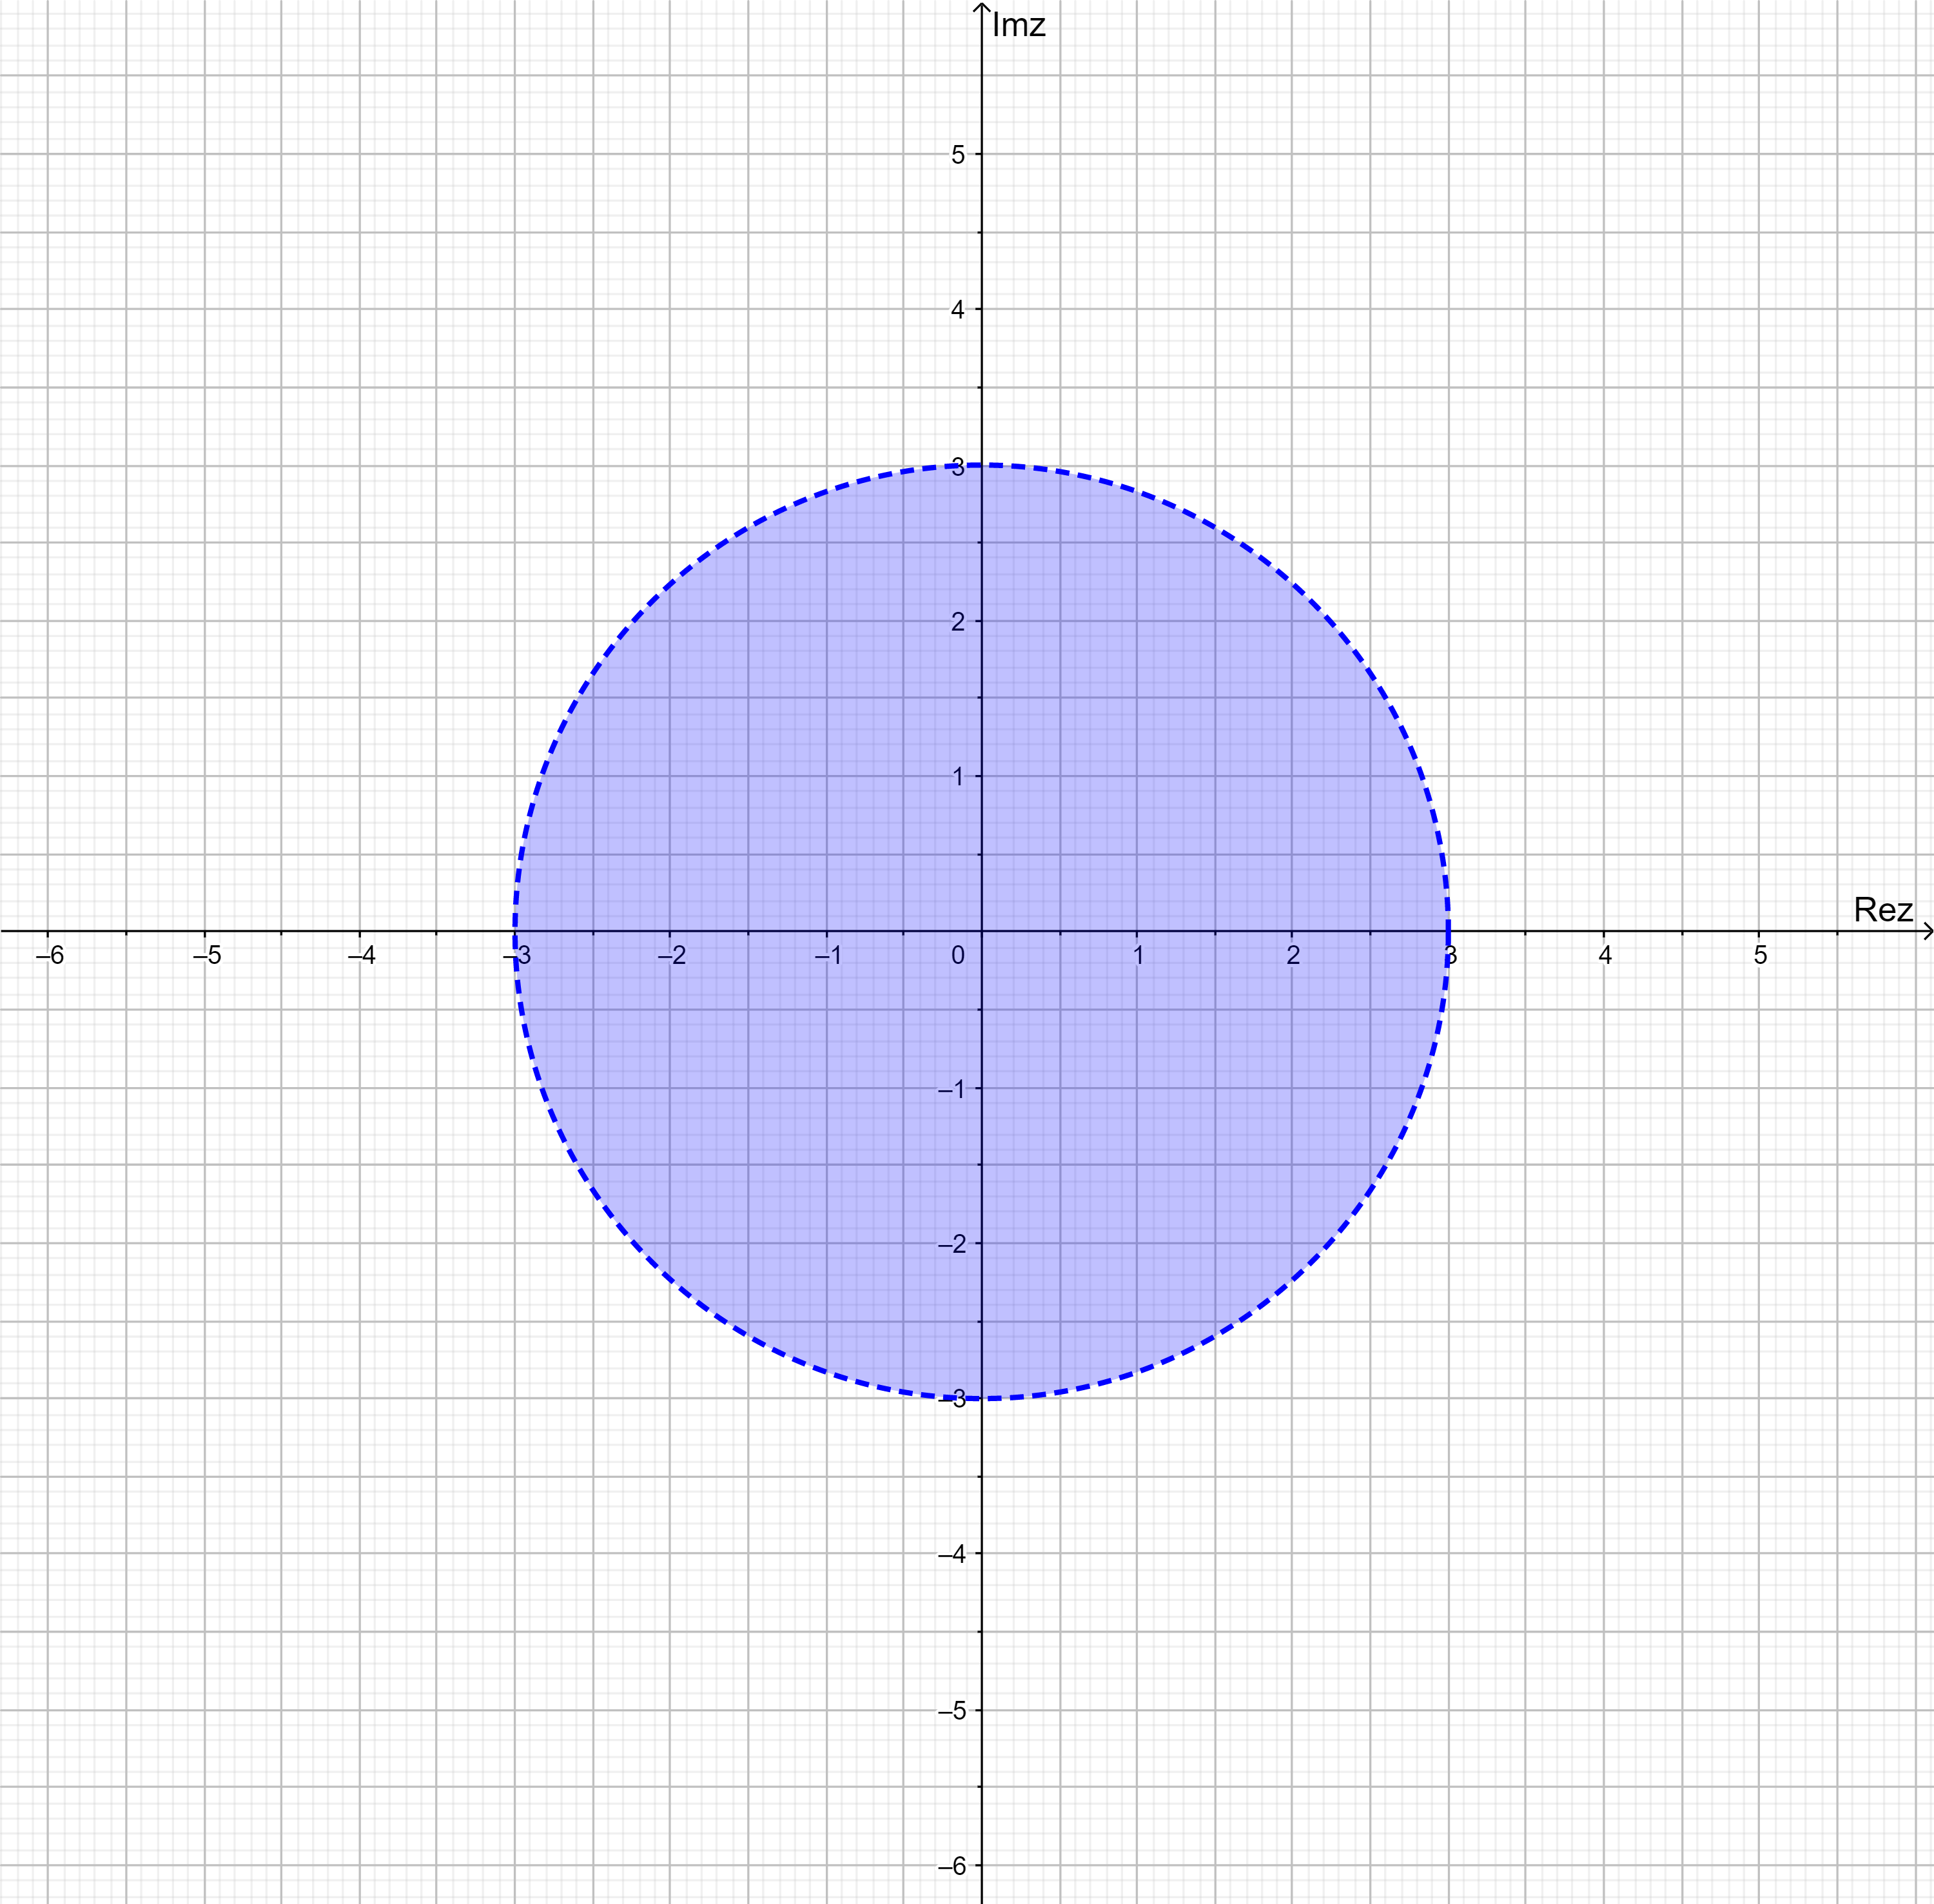
\includegraphics[width=0.75\textwidth]{task4-d.png}
            \caption{Графическое изображение $|z| < 3$}
        \end{figure}\newpage
        \item [e)] $2 < |z + 3 - i| < 3$\\
        Пусть $z = x + iy$. Тогда:\\
        \begin{math}
            2 < |z + 3 - i| < 3 \Leftrightarrow\\\Leftrightarrow
            2 < |x + iy + 3 - i| < 3\Leftrightarrow\\\Leftrightarrow
            2 < |x + 3 + i(y - 1)| < 3\Leftrightarrow\\\Leftrightarrow
            2 < \sqrt{(x + 3)^2 + (y - 1)^2} < 3\Leftrightarrow\\\Leftrightarrow
            2^2 < (x + 3)^2 + (y - 1)^2 < 3^2\Leftrightarrow\\\Leftrightarrow
            4 < (x + 3)^2 + (y - 1)^2 < 9    
        \end{math}\\
        Графическим изображением данного неравенства будет кольцо
        с центром в точке $(-3;1)$, малым радиусом 2 и большим радиусом 3.\\
        \begin{figure}[h]
            \centering
            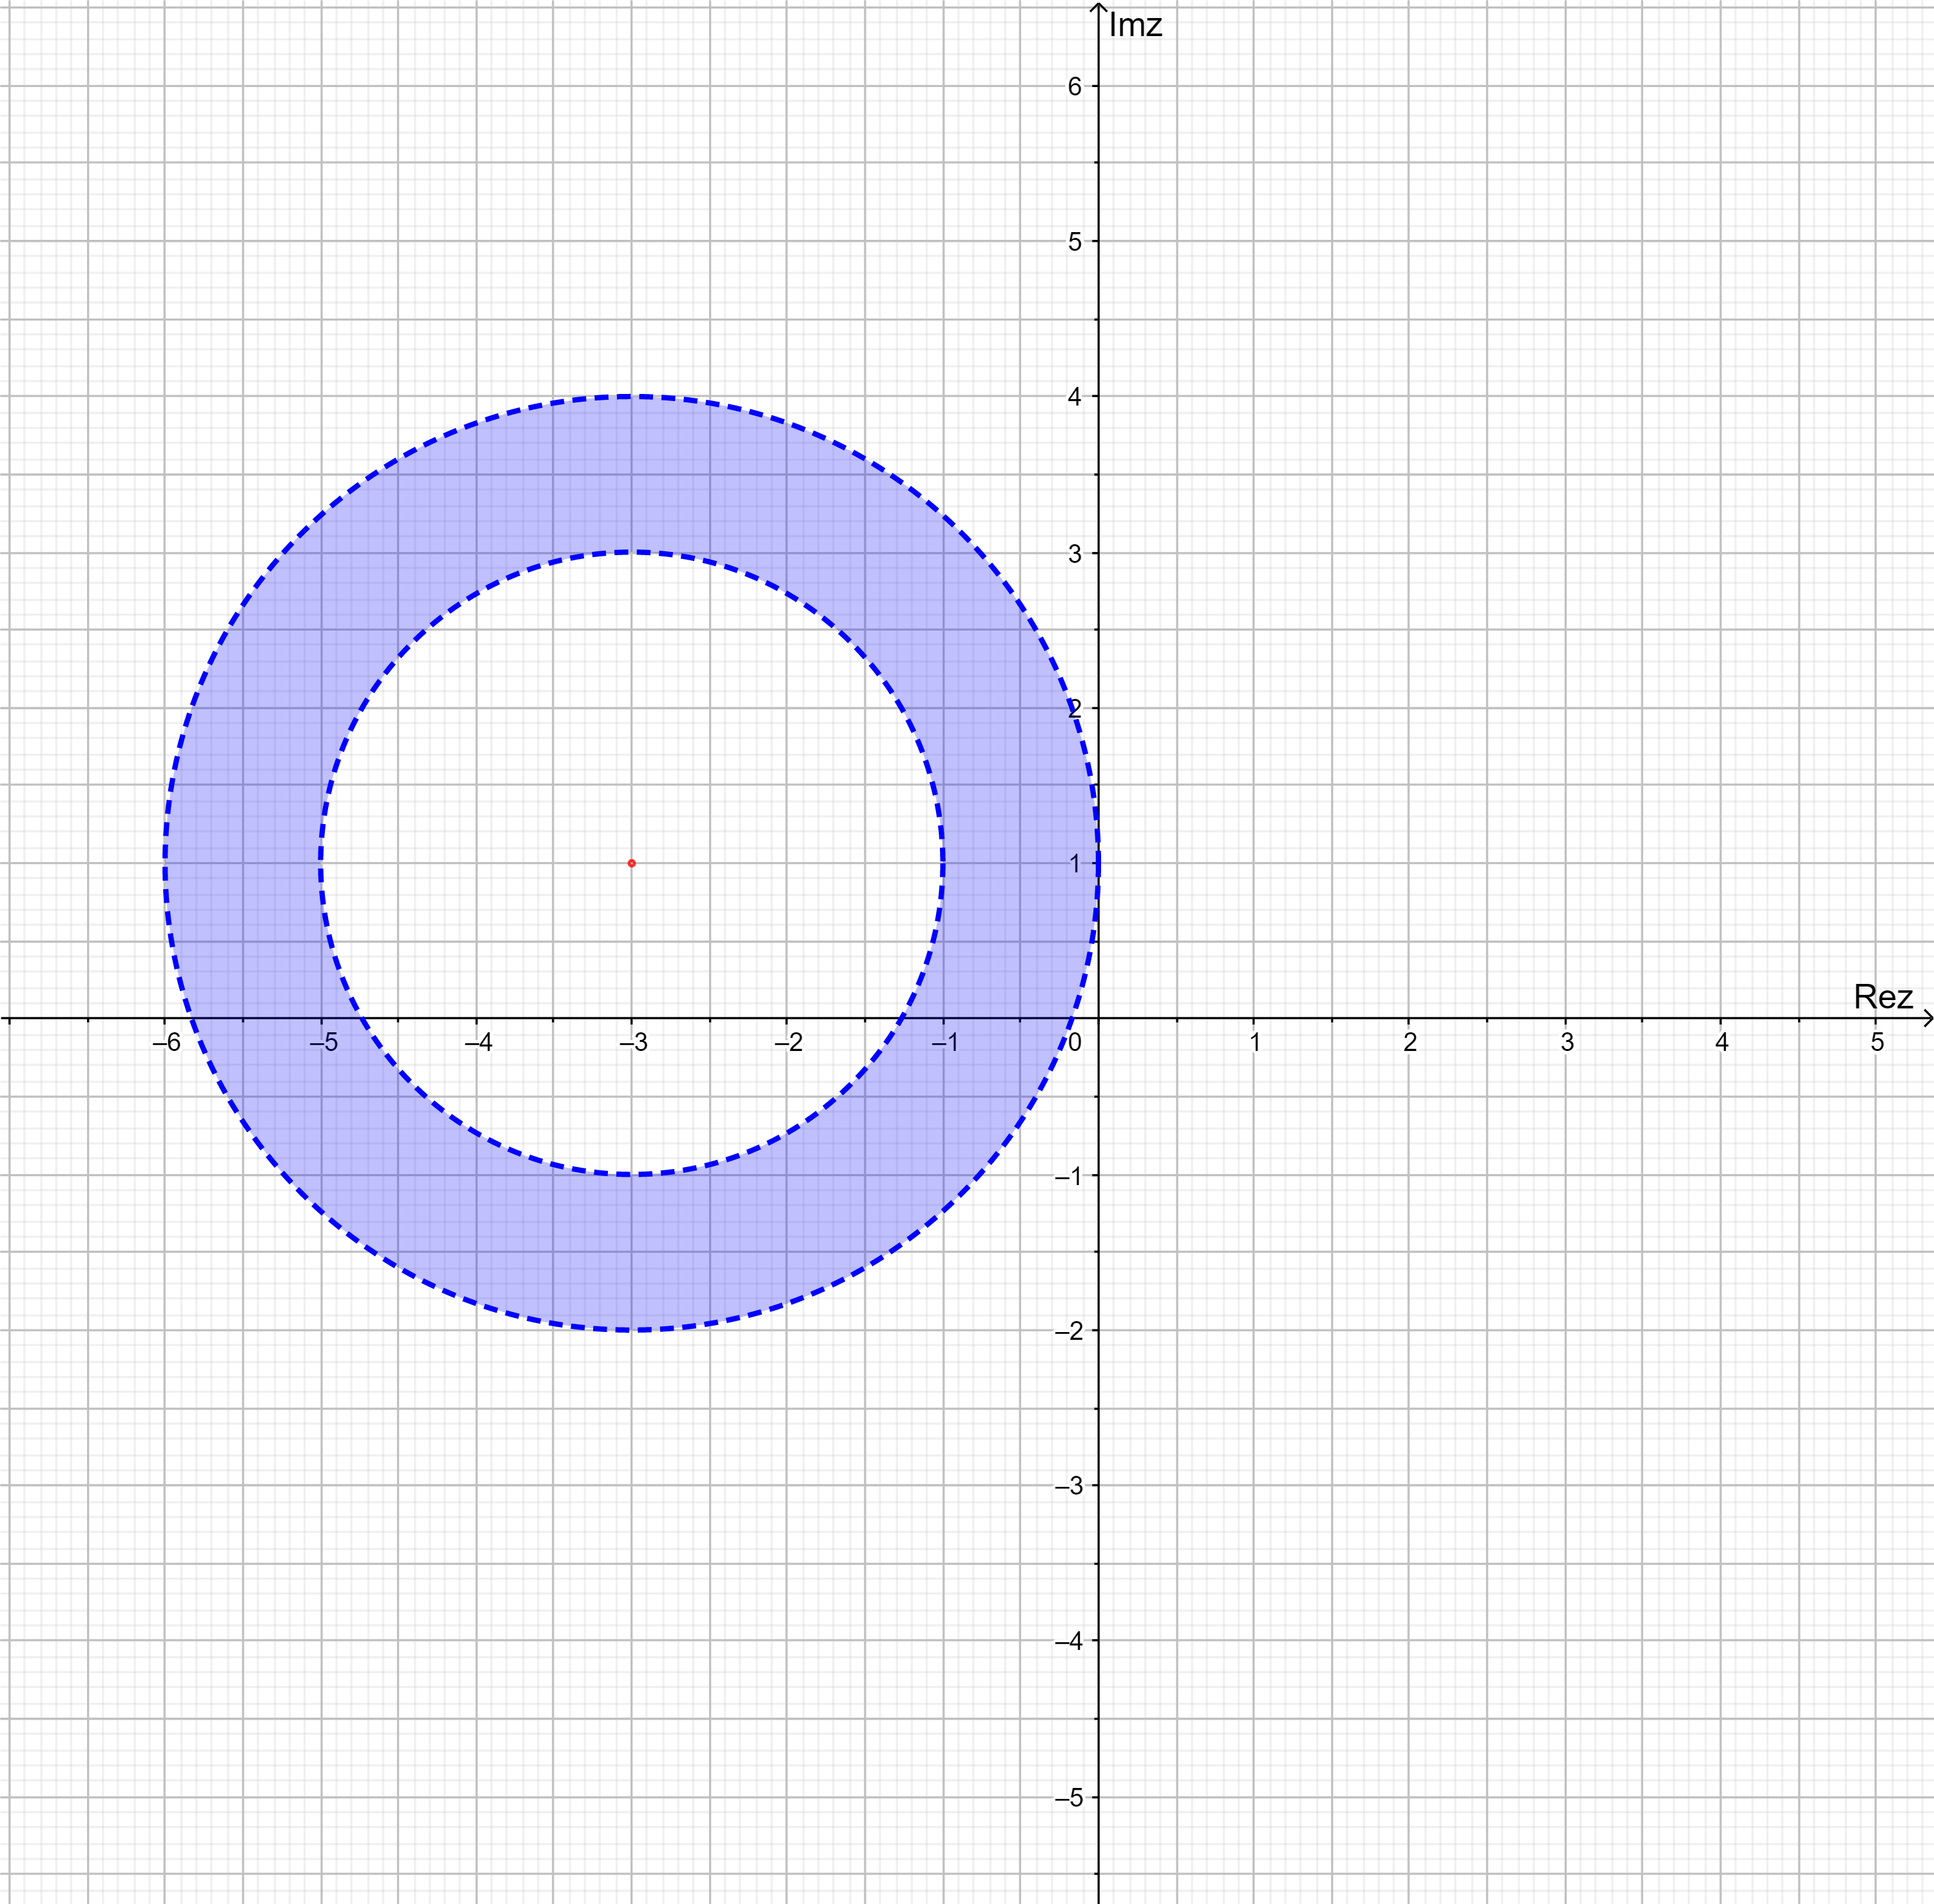
\includegraphics[width=0.75\textwidth]{task4-e.png}
            \caption{Графическое изображение $2 < |z + 3 - i| < 3$}
        \end{figure}\newpage
        \item [f)] $\frac{5\pi}{4} < \arg z < \frac{3\pi}{2}$\\
        Графическим изображением данного неравенства будет
        бесконечный сектор на плоскости, ограниченный двумя прямыми 
        (в третьей четверти, так как отрезок $(\frac{5\pi}{4} ; \frac{3\pi}{2})$
         целиком лежит в третьей четверти):\\
        $y = \arctan(\frac{5\pi}{4})x$ или $y = x$; и\\
        $x = 0$ (поскольку функция арктангенса не оперделена в точке $\frac{3\pi}{2}$)\\\\
        Также стоит отметить, что точка $(0, 0)$ не входит в график, так как
        аргумент числа $z = 0$ не определён. 
        
        \begin{figure}[h]
            \centering
            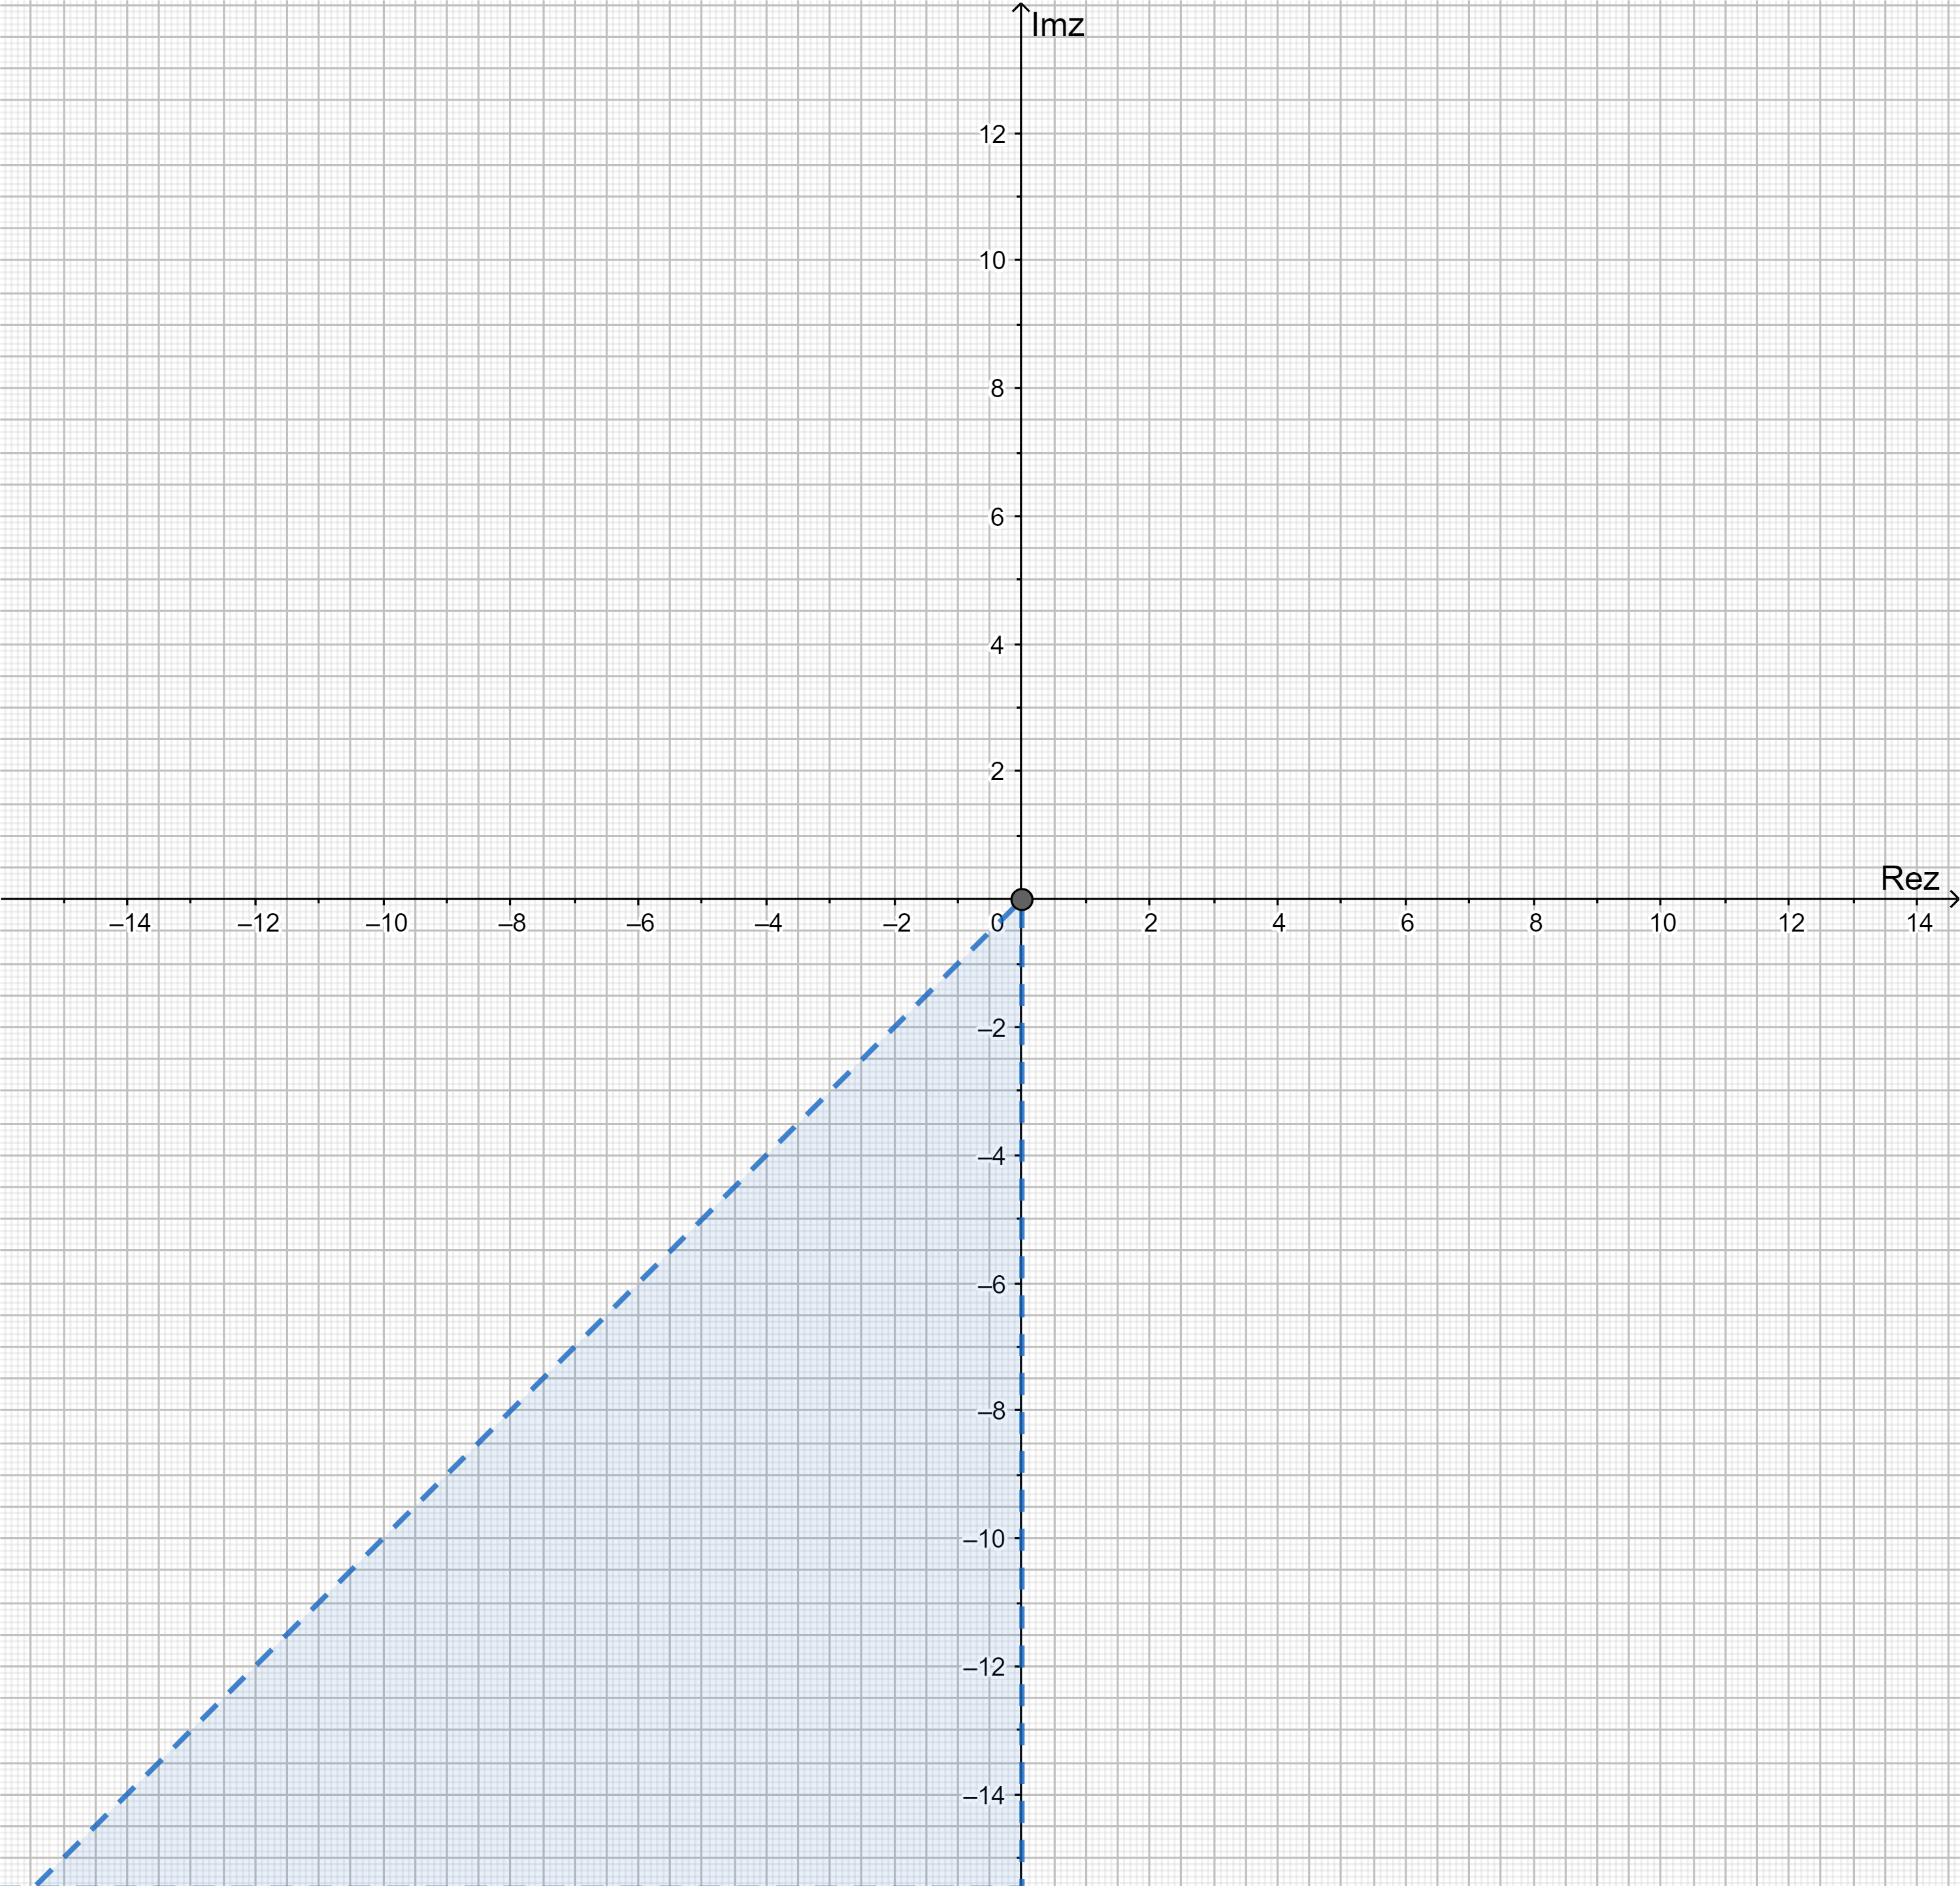
\includegraphics[width=0.75\textwidth]{task4-f.png}
            \caption{Графическое изображение $\frac{5\pi}{4} < \arg z < \frac{3\pi}{2}$}
        \end{figure}
    \end{enumerate}
%--------------------------------------
%
% 5 задание
%
%--------------------------------------
\newpage
\section{Задание.}
    Выполнить разложение на простейшие дроби неправильной рациональной дроби:\\
    $R(z) = \frac{z^5 - 7z^4 + 11z^3 - 5z^2}{4z^3 + 5z^2 - 23z - 6}$
    \subsection*{решение:}
    Поскольку степень числителя больше степени знаменателя, сначала
    нужно выделить целую часть. Для этого
    выполним деление числителя на знаменатель в столбик:\\\\
    \begin{spacing}{1.4}
        \begin{tabular}{*{15}{cp{0.55cm}}}
            &$z^5$             & $-$ & $7z^4$            & $+$ & $11z^3$             & $-$ & $5z^2$               &\vline   
            $4z^3$            & $+$ & $5z^2$            & $-$ & $23z$               & $-$ & $6$\\
            \cline{1-1}\cline{9-15}
            &$z^5$             & $+$ & $\frac{5}{4}z^4$  & $-$ & $\frac{23}{4}z^3$   & $-$ & $\frac{3}{2}z^2$     &\vline
            $\frac{1}{4}z^2$  & $-$ & $\frac{33}{16}z$  & $+$ & $\frac{433}{64}$    &     &\\
            \cline{2-8}
            &                  & $-$ & $\frac{33}{4}z^4$ & $+$ & $\frac{67}{4}z^3$   & $-$ & $\frac{7}{2}z^2$     &
                              &     &                   &     &                     &     &\\
            \cline{1-1}
            &                  & $-$ & $\frac{33}{4}z^4$ & $-$ & $\frac{165}{16}z^3$ & $+$ & $\frac{759}{16}z^2$  &
            $+$               & $\frac{99}{8}z$    &    &     &                     &     &\\
            \cline{4-10}
            &                  &     &                   &     & $\frac{433}{16}z^3$ & $-$ & $\frac{615}{15}z$    &
            $-$               & $\frac{99}{8}$     &    &     &                     &     &\\
            \cline{1-1}
            &                  &     &                   &     & $\frac{433}{16}z^3$ & $+$ & $\frac{2165}{64}z^2$ &
            $-$               & $\frac{9959}{64}z$ &    & $-$ & $\frac{2598}{64}$   &     &\\
            \cline{6-13}
            &                  &     &                   &     &                     & $-$ & $\frac{5425}{64}z^2$ &
            $+$               & $\frac{9167}{64}z$ &    & $+$ & $\frac{2598}{64}$   &     &\\
        \end{tabular}\\\\ 
    \end{spacing}
    %
    %
    В результате деления получаем:\\
    \begin{math}
        R(z) = \frac{1}{4}z^2 + \frac{33}{16}z + \frac{433}{64} +
        \frac{-\frac{5425}{64}z^2 + \frac{9167}{64}z + \frac{2598}{64}}
        {4z^3 + 5z^2 - 23z - 6}
    \end{math}\\\\
    Нам остаётся выполнить разложение правильной рациональной дроби\\
    $M(z) = \frac{-\frac{5425}{64}z^2 + \frac{9167}{64}z + \frac{2598}{64}}
    {4z^3 + 5z^2 - 23z - 6}$\\\\
    Теперь разложим знаменатель. Поскольку у нас полином третьей степени,
    стоит сначала попробовать найти целый корень с помощью схемы Горнера. 
    Делители свободного члена
    $6: 1, -1, 2, -2, 3, -3, 6, -6$. Начнём перебор с 1:\\
    \begin{tabular}{|c|c|c|c|c|}
        \hline
            & 4 & 5 & -23 & -6\\
        \hline
        1   & 4 & 9 & -14 & -20\\
        \hline
        -1  & 4 & 5 & -19 & -1\\
        \hline
        2   & 4 &13 &  3  & 0\\
        \hline
    \end{tabular}\\\\
    $b_3 = 0$, значит 2 - корень. Таким образом,\\
    $4z^3 + 5z^2 - 23z - 6 = (z - 2)(4z^2 + 13z + 3)$
    Остаётся решить квадратное уравнение $4z^2 + 13z + 3$. Решим его
    через дискриминант:\\
    \begin{math}
        D = b^2 - 4ac = 13^2 - 4\cdot4\cdot3 = 169 - 48 = 121 = 11^2
        z_{1,2} = \frac{-b\pm \sqrt{D}}{2a} = \frac{-13\pm \sqrt{11^2}}{8}\\
        z_1 = -3, z_2 = -\frac{1}{4}
    \end{math}\\\\
    Таким образом, разложение знаменателя на множители выглядит так:\\
    $(z - 2)(z + 3)(4z + 1)$\\
    Тогда $M(z)$ примет вид:\\\\
    $M(z) = \frac{-\frac{5425}{64}z^2 + \frac{9167}{64}z + \frac{2598}{64}}
    {(z - 2)(z + 3)(4z + 1)}$\\\\
    Можно заметить, что если поделить числитель и знаменатель на 4, все множители
    разложения знаменателя станут неприводимыми линейными. Тогда можно применить
    формулу Лагранжа:\\
    \[ \frac{f(z)}{g(z)} = \sum_{k=1}^{n} \frac{f(z_k)}{g'(z_k)(z-z_k)} \].\\
    В нашем случае:
    $f(z) = -\frac{5425}{256}z^2 + \frac{9167}{256}z + \frac{2598}{256}$ и\\\\
    $g(z) = (z - 2)(z + 3)(z + \frac{1}{4}) = z^3 + \frac{5}{4}z^2 - \frac{23}{4}z - \frac{3}{2}$\\\\
    Найдём производную $g(x)$.\\
    \begin{math}
        g'(z) = (z^3 + \frac{5}{4}z^2 - \frac{23}{4}z)' = (z^3)' + (\frac{5}{4}z^2)' - (\frac{23}{4}z)' = \\
        3z^2 + 2\cdot\frac{5}{4}z - \frac{23}{4} - 0 = 3z^2 + \frac{5}{2}z - \frac{23}{4}
    \end{math}\\\\
    Подставим найденные значения в формулу Лагранжа.
    Таким образом, $M(z)$ примет следующий вид:\\
    \begin{math}
        M(z) = \frac{f(2)}{g'(2)(z - 2)} + 
        \frac{f(-3)}{g'(-3)(z + 3)} +
        \frac{f(-\frac{1}{4})}{g'(-\frac{1}{4})(z + \frac{1}{4})} =\\\\
        = 
        \frac{-\frac{5425}{256}(2)^2 + \frac{9167}{256}(2) + \frac{2598}{256}}
            {(3\cdot(2)^2 + \frac{5}{2}\cdot(2) - \frac{23}{4})(z-2)} + 
        \frac{-\frac{5425}{256}(-3)^2 + \frac{9167}{256}(-3) + \frac{2598}{256}}
            {(3\cdot(-3)^2 + \frac{5}{2}\cdot(-3) - \frac{23}{4})(z+3)} + 
        \frac{-\frac{5425}{256}(-\frac{1}{4})^2 + \frac{9167}{256}(-\frac{1}{4}) + \frac{2598}{256}}
            {(3\cdot(-\frac{1}{4})^2 + \frac{5}{2}\cdot(-\frac{1}{4}) - \frac{23}{4})(z+\frac{1}{4})} =\\\\
        =
        \frac{-\frac{5425}{64} + \frac{9167}{128} + \frac{2598}{256}}
        {(12 + 5 - \frac{23}{4})(z - 2)} +
        \frac{-\frac{48825}{256} - \frac{27501}{256} + \frac{2598}{256}}
        {(27 - \frac{15}{2} - \frac{23}{4})(z + 3)} +
        \frac{-\frac{5425}{4096} - \frac{9167}{1024} + \frac{2598}{256}}
        {\frac{3}{16} - \frac{5}{8} - \frac{23}{4}}=\\\\
        =
        \frac{-3}{\frac{45}{4}(z - 2)} -
        \frac{-288}{\frac{55}{4}(z + 3)} +
        \frac{-\frac{525}{4096}}{-\frac{99}{16}(z + \frac{1}{4})}=\\\\
        =
        -\frac{4}{15(z-2)} - \frac{1152}{55(z + 3)} + \frac{175}{2112(4z + 1)}
    \end{math}
    \subsection*{Ответ:}
    \begin{math}
        R(z) = \frac{1}{4}z^2 + \frac{33}{16}z + \frac{433}{64} -
        \frac{4}{15(z-2)} - \frac{1152}{55(z + 3)} + \frac{175}{2112(4z + 1)}
    \end{math}
\end{document}